\section{A Characterization Study on the First Run~\label{sec:sodb9_r3_hist}} 
This section further discusses the first run of 
INC with its task length increasing from 1 second to 4096 seconds via EMPv5 with no Step 2. 
The detailed description of the base data is from Table~\ref{tab:exp_notes3}.

%\begin{table}[h]
%\begin{center}
%\begin{tabular}{|p{2cm}|p{3cm}|p{3cm}|p{4cm}|p{3.5cm}|} \hline
%Machine & Task Length (sec) & Description & Experiment Period & Relevant \linebreak Histograms\\ \hline
%{\tt sodb9} &  INC1$\sim$INC64 & 1000 samples, each & 2017-03-13 $\sim$ 2017-03-14 & %Figs.~\ref{fig:s9_r2_et_hist1},~\ref{fig:s9_r2_et_hist2},~\ref{fig:s9_r2_pt_hist1}, and~\ref{fig:s9_r2_pt_hist2}\\ \hline
%{\tt sodb9} &  INC512$\sim$INC1024 & 300 samples, each & 2017-03-17 $\sim$ 2017-03-21 & 
%%Figs.~\ref{fig:s9_r2_et_hist3} and~\ref{fig:s9_r2_pt_hist3}\\ \hline
%{\tt sodb10} & INC2048 & 300 samples & 2017-03-13 $\sim$ 2017-03-20 & 
%%Figs.~\ref{fig:inc2048_r2_et_hist_v5} and~\ref{fig:inc2048_r2_hist_v5}\\ \hline
%{\tt sodb12} & INC4096 & 300 samples & 2017-03-02 $\sim$ 2017-03-17 & 
%%Figs.~\ref{fig:inc4096_r2_et_hist_v5} and~\ref{fig:inc4096_r2_hist_v5}\\ \hline
%{\tt sodb10} & INC8192& 261 samples & 2017-04-27 $\sim$ 2017-05-21 & 
%%Figs.~\ref{fig:inc8192_r2_et_hist_v5} and~\ref{fig:inc8192_r2_hist_v5}\\ \hline
%{\tt sodb12} & INC16384& 130 samples & 2017-04-27 $\sim$ 2017-05-21 & 
%%Figs.~\ref{fig:inc16384_r2_et_hist_v5} and~\ref{fig:inc16384_r2_hist_v5}\\ \hline
%\end{tabular}
%\end{center}
%\vspace{-.2in}
%\caption{Notes on experiment runs used for histograms\label{tab:exp_notes3}}
%\end{table}
%
%INC8192/INC16384 unfortunately stopped in the middle of their runs due to a frozen vnc problem. So couldn't finish 300 samples.
%
%\pagebreak

\subsection{Summary of Histograms}

\begin{figure}[hp!]
\vspace{-.3in}
	\centering
	\includegraphics[scale=0.5,angle=270]{u_s_time/3d_plot.eps}\label{fig:3d_plot}
	\caption{3D histograms on INC~\label{fig:hist3d}}
\end{figure}

\subsection{Absolute and Relative Variance over Increasing Task Length}

\begin{figure}[hp!]
	\centering
	\subfigure[Standard deviation (absolute)]{
		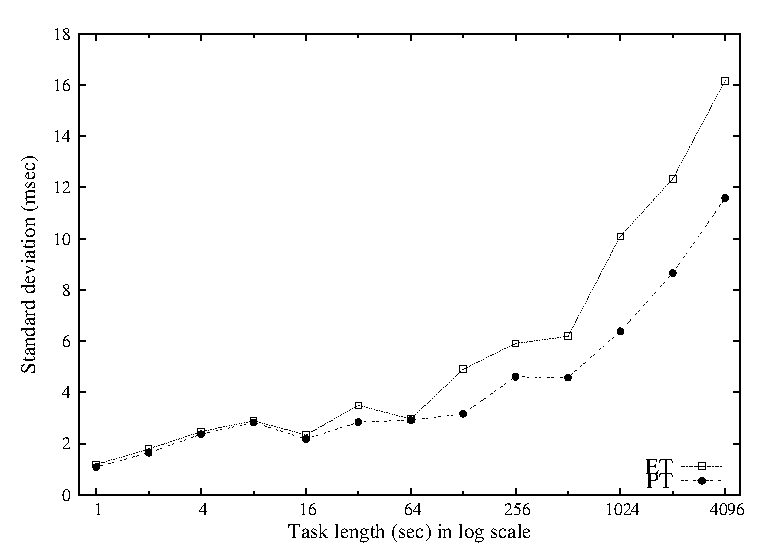
\includegraphics[scale=0.6]{u_s_time/overall_std.eps}
		\label{fig:overall_std}
	}
	\subfigure[Coefficient of variation (relative)]{
		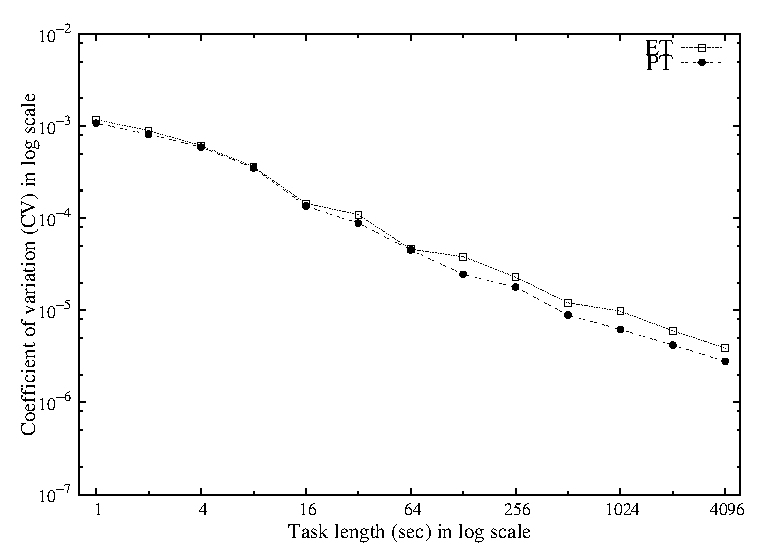
\includegraphics[scale=0.6]{u_s_time/overall_re.eps}
		\label{fig:overall_re}
	}
	\caption{Absolute and relative variances~\label{fig:cv_inc}}
\end{figure}

\pagebreak
\newpage

\subsection{ET}

\begin{figure}[hp!]
	\centering
	\subfigure[ET frequency on INC1]{
		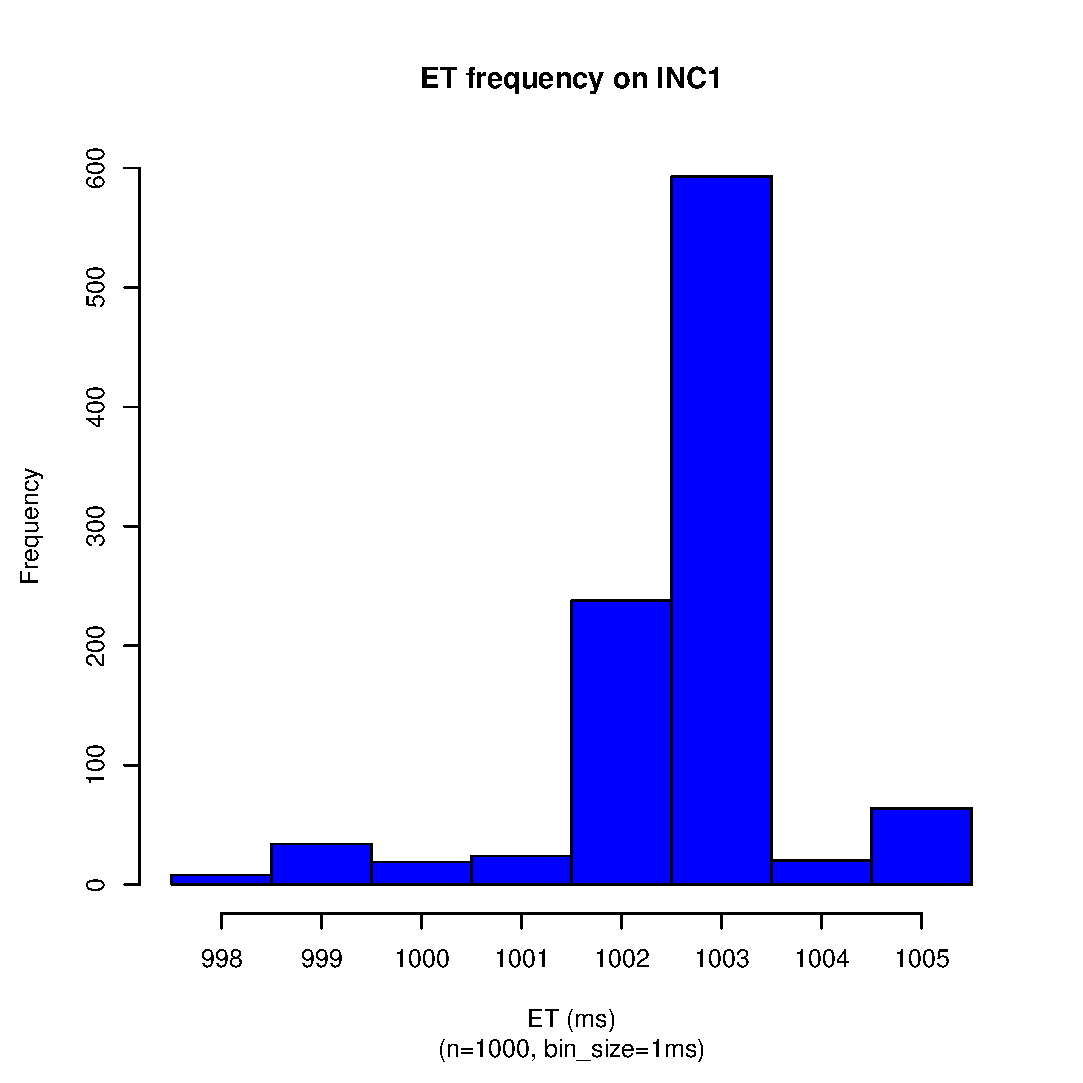
\includegraphics[scale=0.43]{u_s_time/1_sec_et_hist.eps}
		\label{fig:inc1_r3_et_hist_v5}
	}
	\subfigure[ET frequency on INC2]{
		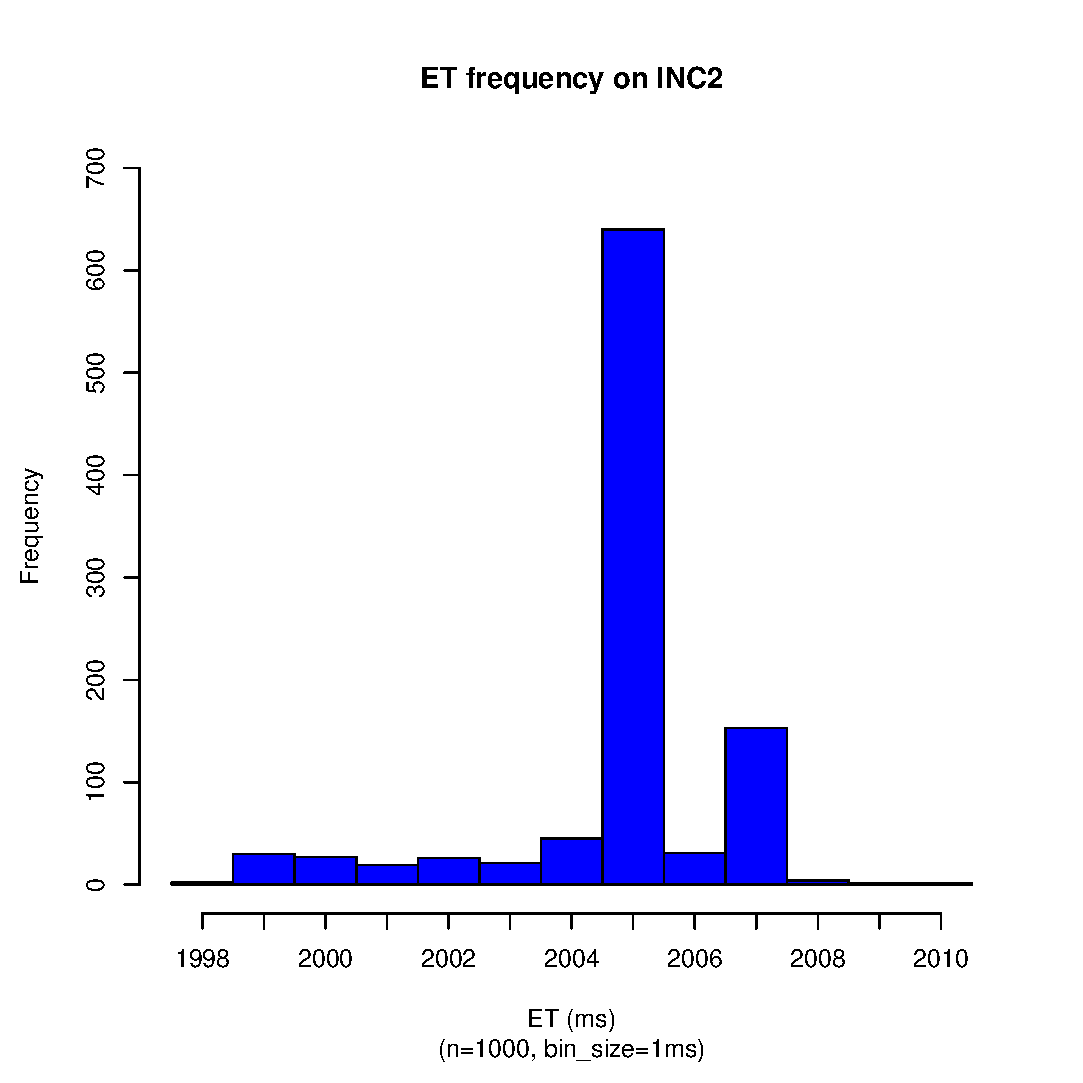
\includegraphics[scale=0.43]{u_s_time/2_sec_et_hist.eps}
		\label{fig:inc2_r3_et_hist_v5}
	}
	\subfigure[ET frequency on INC4]{
		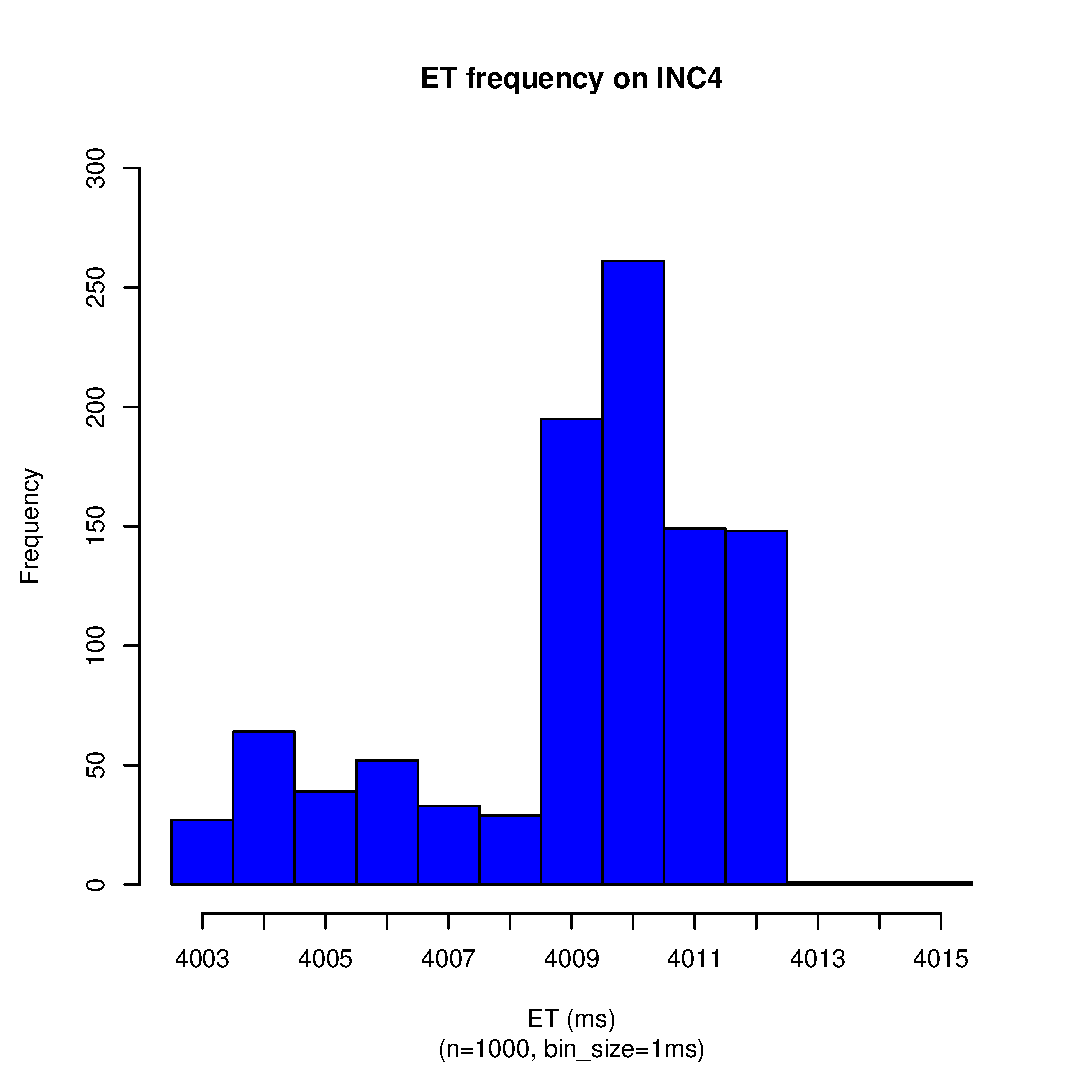
\includegraphics[scale=0.43]{u_s_time/4_sec_et_hist.eps}
		\label{fig:inc4_r3_et_hist_v5}
	}
	\subfigure[ET frequency on INC8]{
		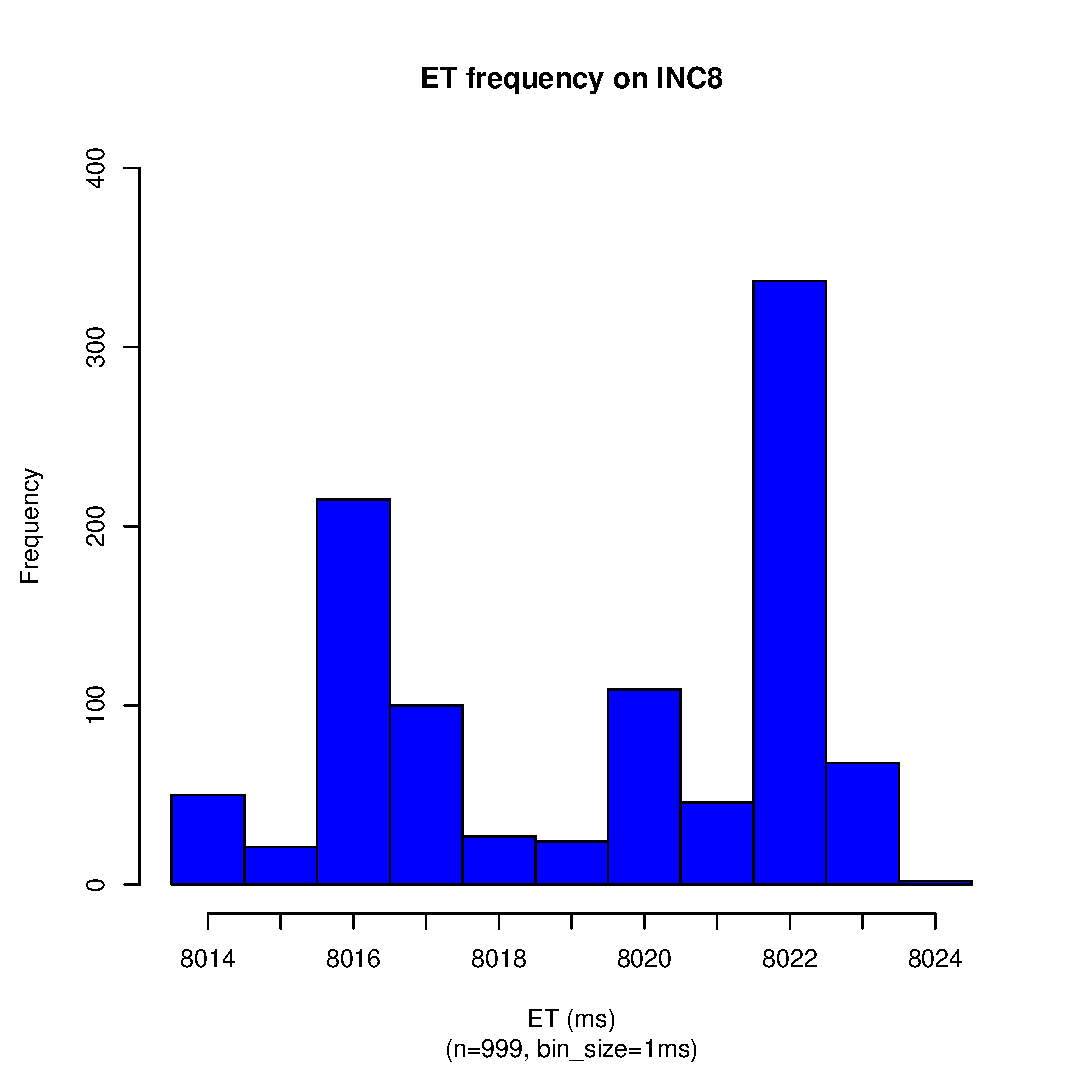
\includegraphics[scale=0.43]{u_s_time/8_sec_et_hist.eps}
		\label{fig:inc8_r3_et_hist_v5}
	}
	\caption{ET Histograms of INC1 ... INC8~\label{fig:s9_r3_et_hist1}}
\end{figure}

\begin{figure}[hp!]
	\centering
	\subfigure[ET frequency on INC16]{
		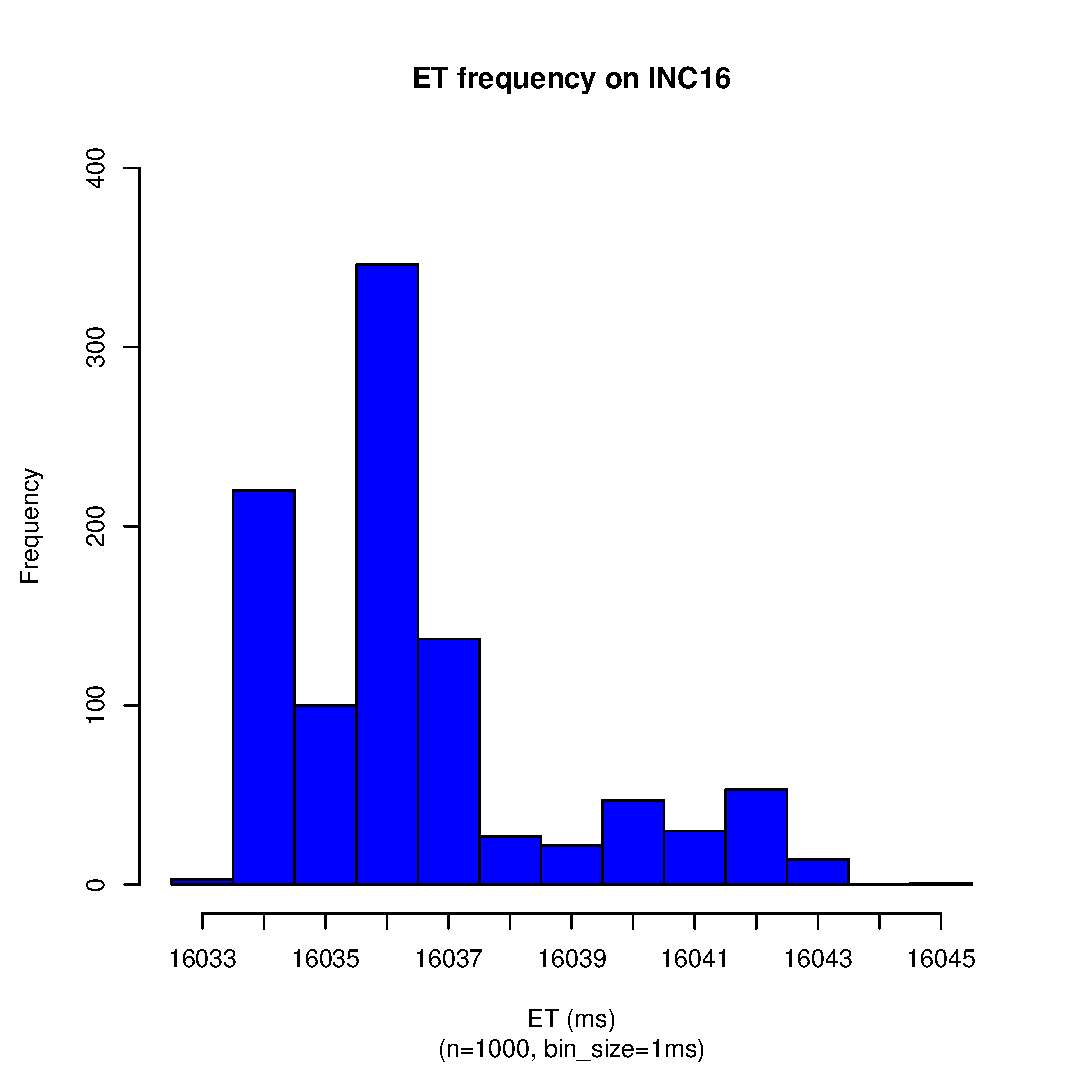
\includegraphics[scale=0.43]{u_s_time/16_sec_et_hist.eps}
		\label{fig:inc16_r3_et_hist_v5}
	}
	\subfigure[ET frequency on INC32]{
		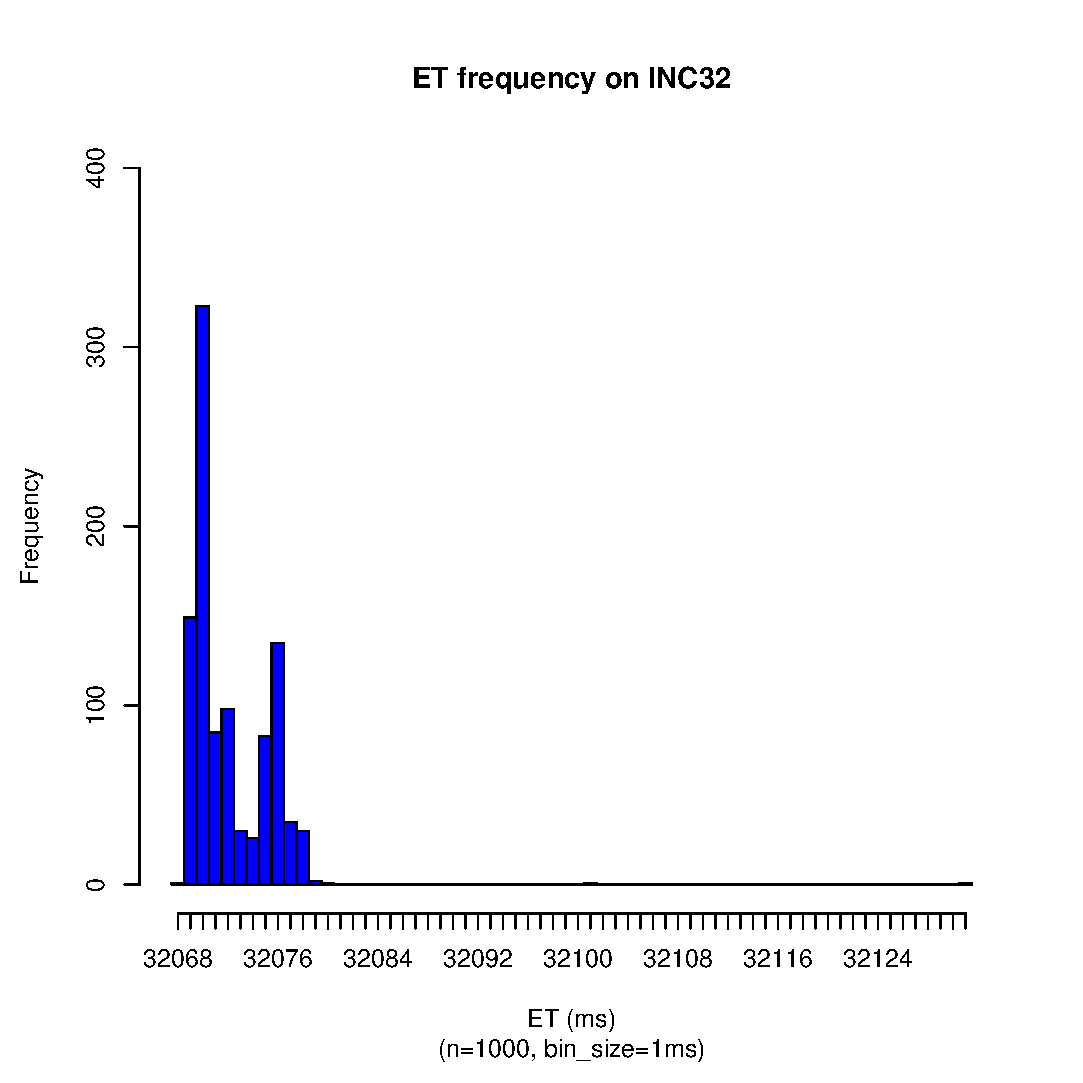
\includegraphics[scale=0.43]{u_s_time/32_sec_et_hist.eps}
		\label{fig:inc32_r3_et_hist_v5}
	}
	\subfigure[ET frequency on INC64]{
		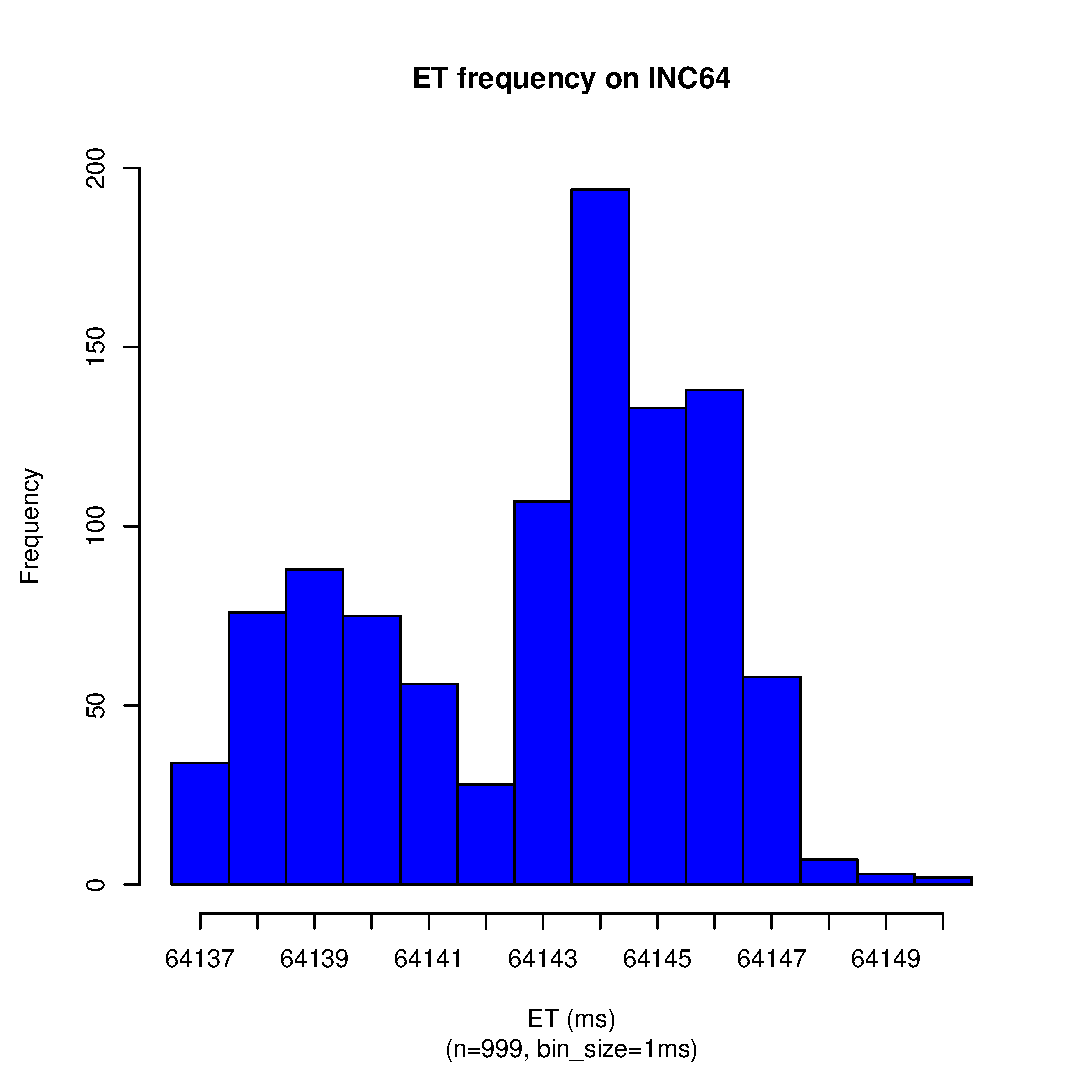
\includegraphics[scale=0.43]{u_s_time/64_sec_et_hist.eps}
		\label{fig:inc64_r3_et_hist_v5}
	}
	\caption{ET Histograms of INC16 ... INC64~\label{fig:s9_r3_et_hist2}}
\end{figure}

\begin{figure}[hp!]
	\centering
	\subfigure[ET frequency on INC128]{
		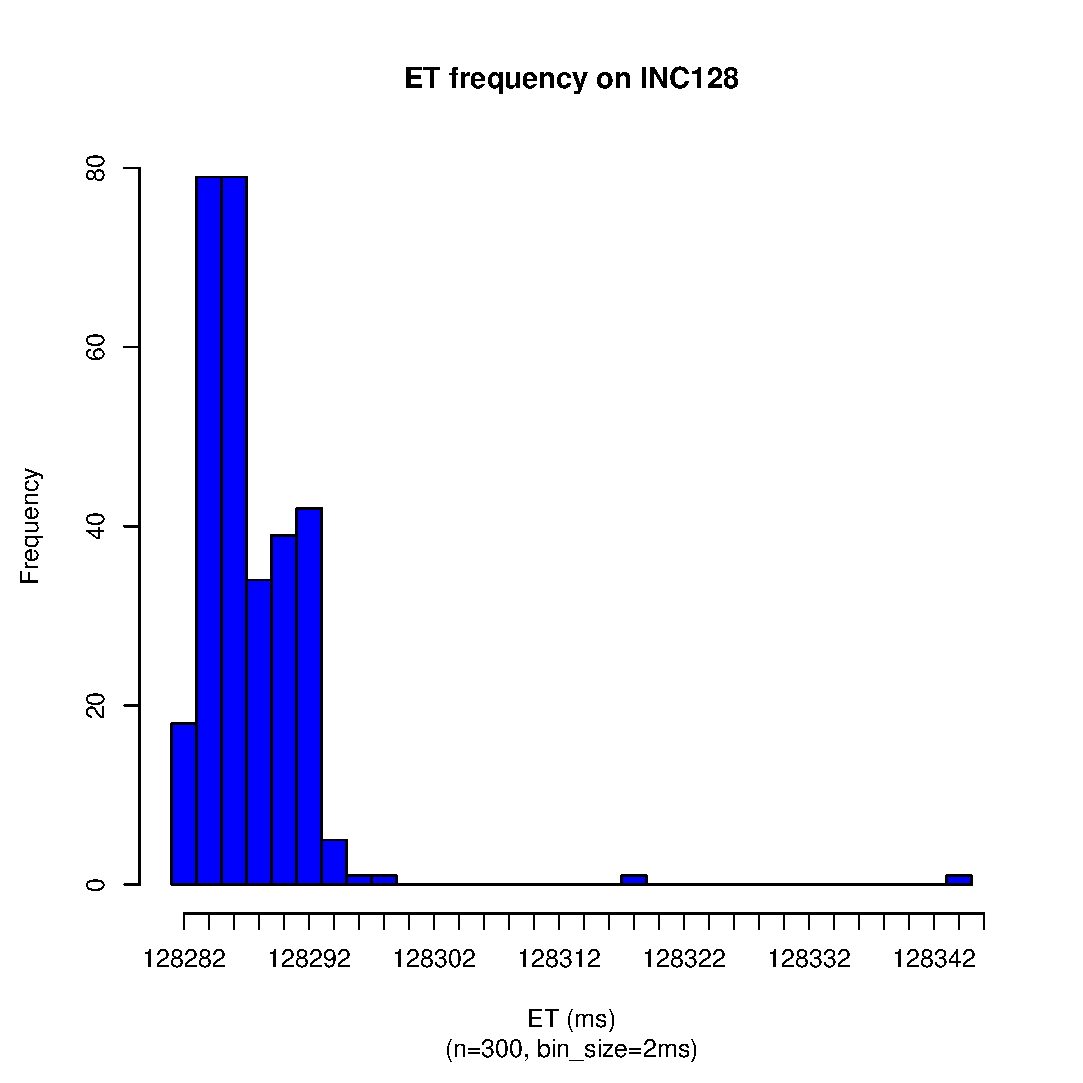
\includegraphics[scale=0.43]{u_s_time/128_sec_et_hist.eps}
		\label{fig:inc128_r3_et_hist_v5}
	}
	\subfigure[ET frequency on INC256]{
		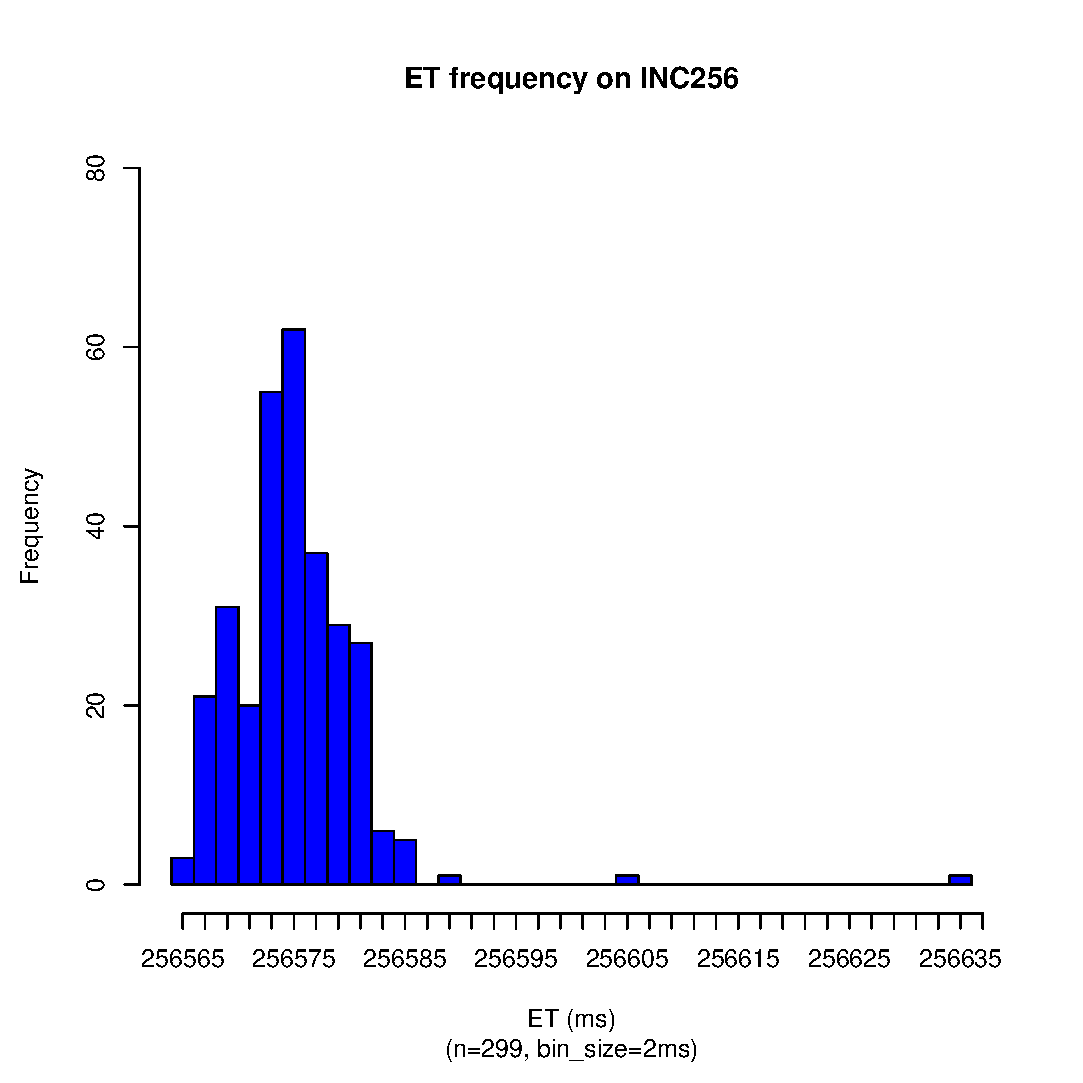
\includegraphics[scale=0.43]{u_s_time/256_sec_et_hist.eps}
		\label{fig:inc256_r3_et_hist_v5}
	}
	\subfigure[ET frequency on INC512]{
		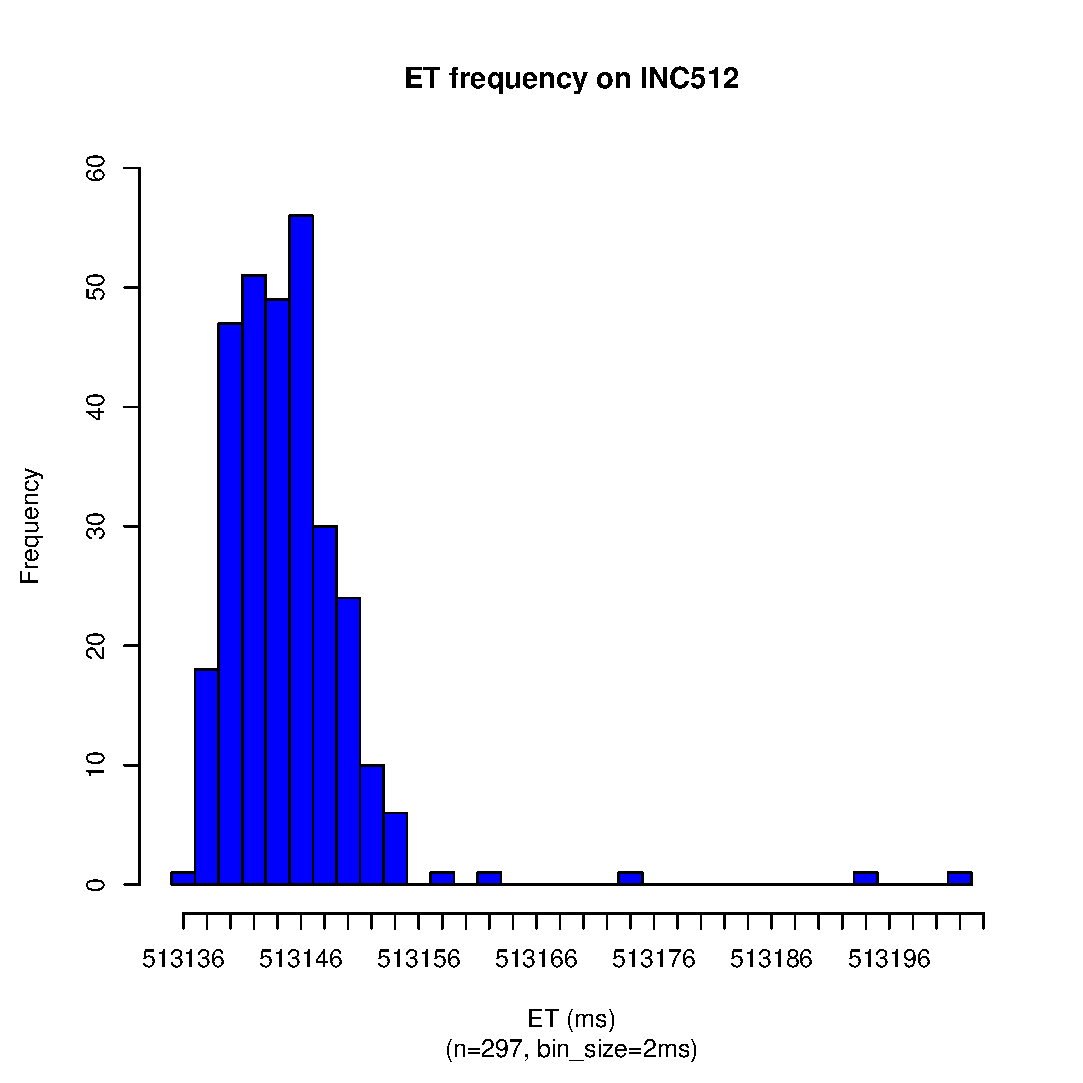
\includegraphics[scale=0.43]{u_s_time/512_sec_et_hist.eps}
		\label{fig:inc512_r3_et_hist_v5}
	}
	\subfigure[ET frequency on INC1024]{
		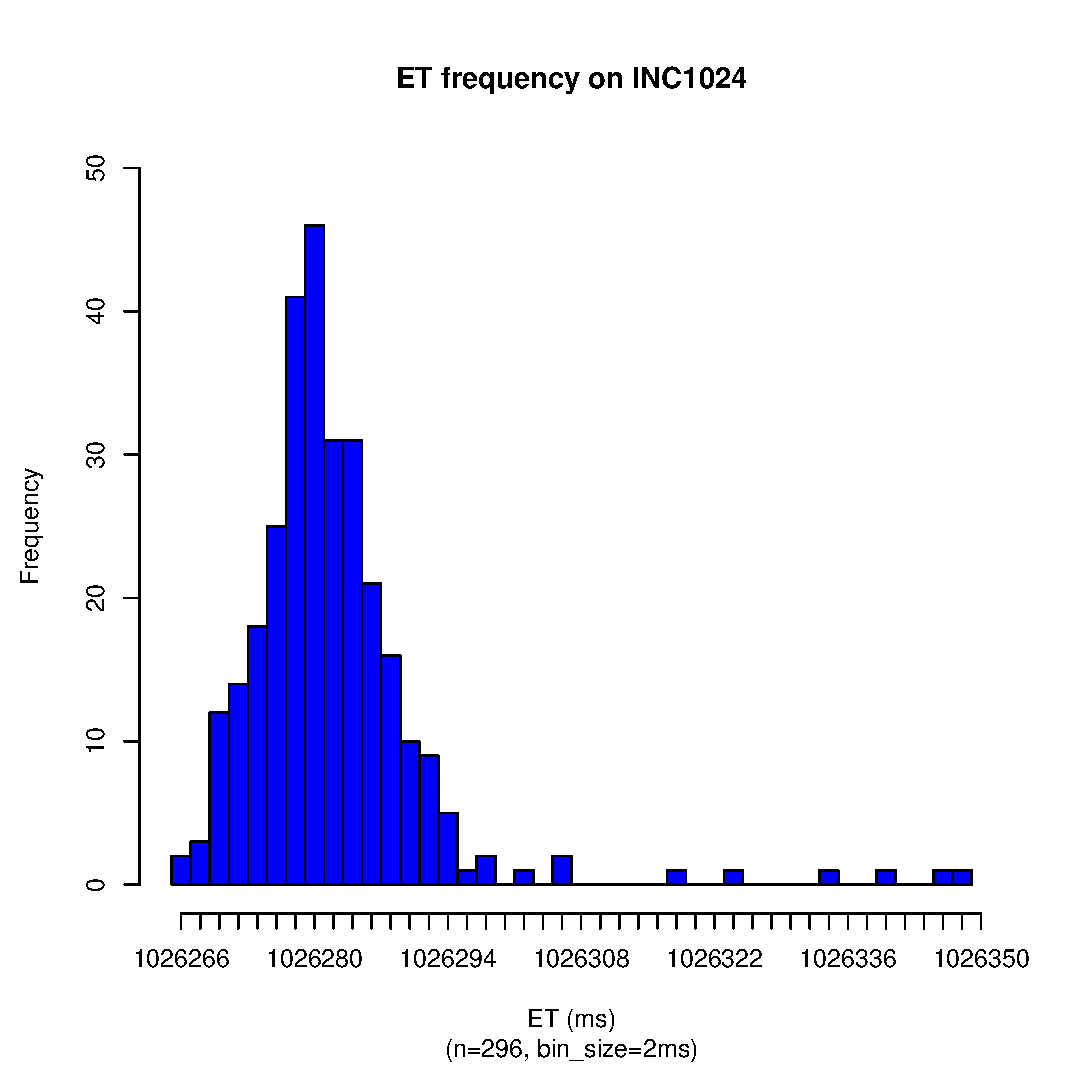
\includegraphics[scale=0.43]{u_s_time/1024_sec_et_hist.eps}
		\label{fig:inc1024_r3_et_hist_v5}
	}
	\caption{ET Histograms of INC128 ... INC1024~\label{fig:s9_r3_et_hist3}}
\end{figure}

%\begin{figure}[hp!]
%	\centering
%	\subfigure[ET frequency on INC2048]{
%		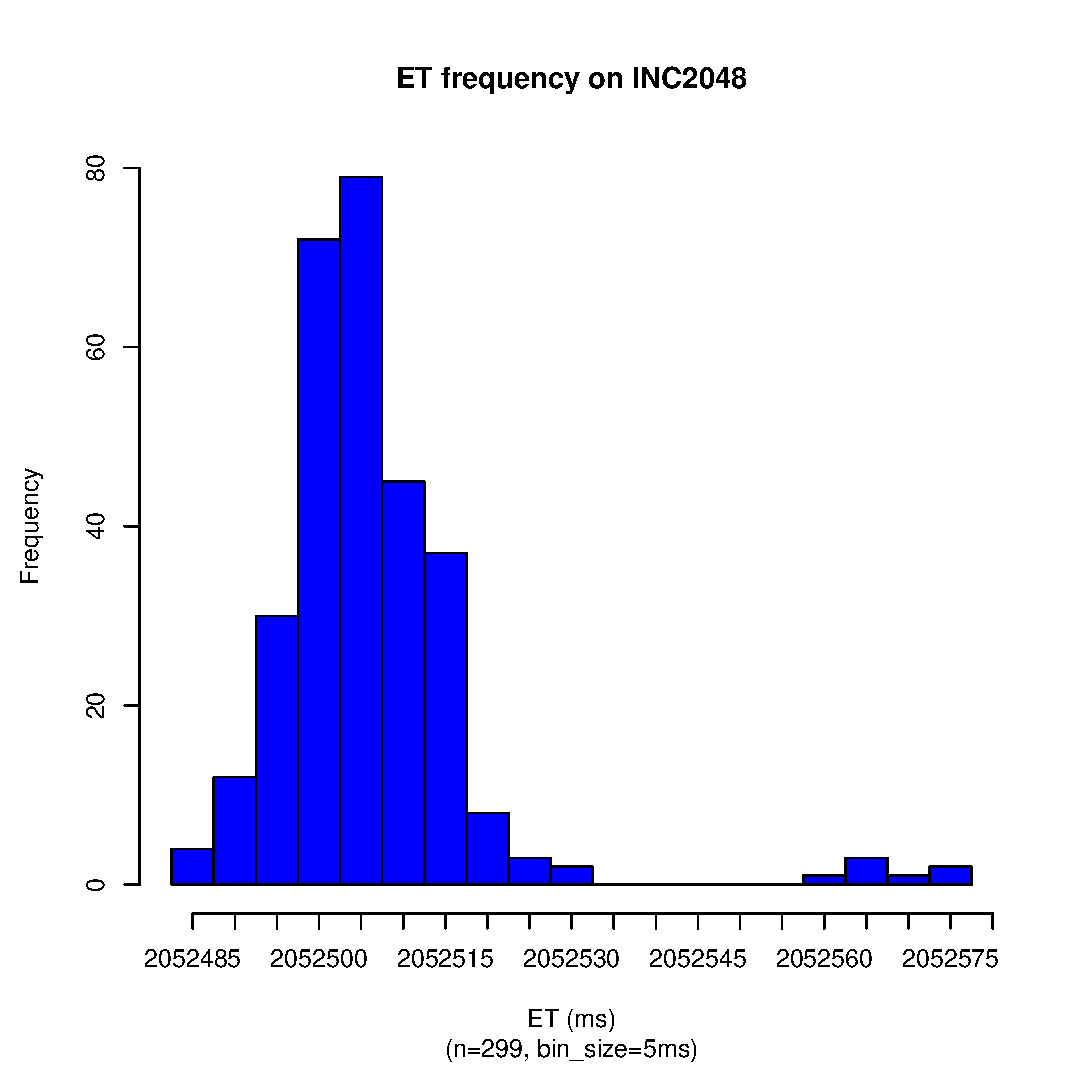
\includegraphics[scale=0.43]{u_s_time/2048_sec_et_hist.eps}
%		\label{fig:inc2048_r3_et_hist_v5}
%	}
%	\subfigure[ET frequency on INC4096]{
%		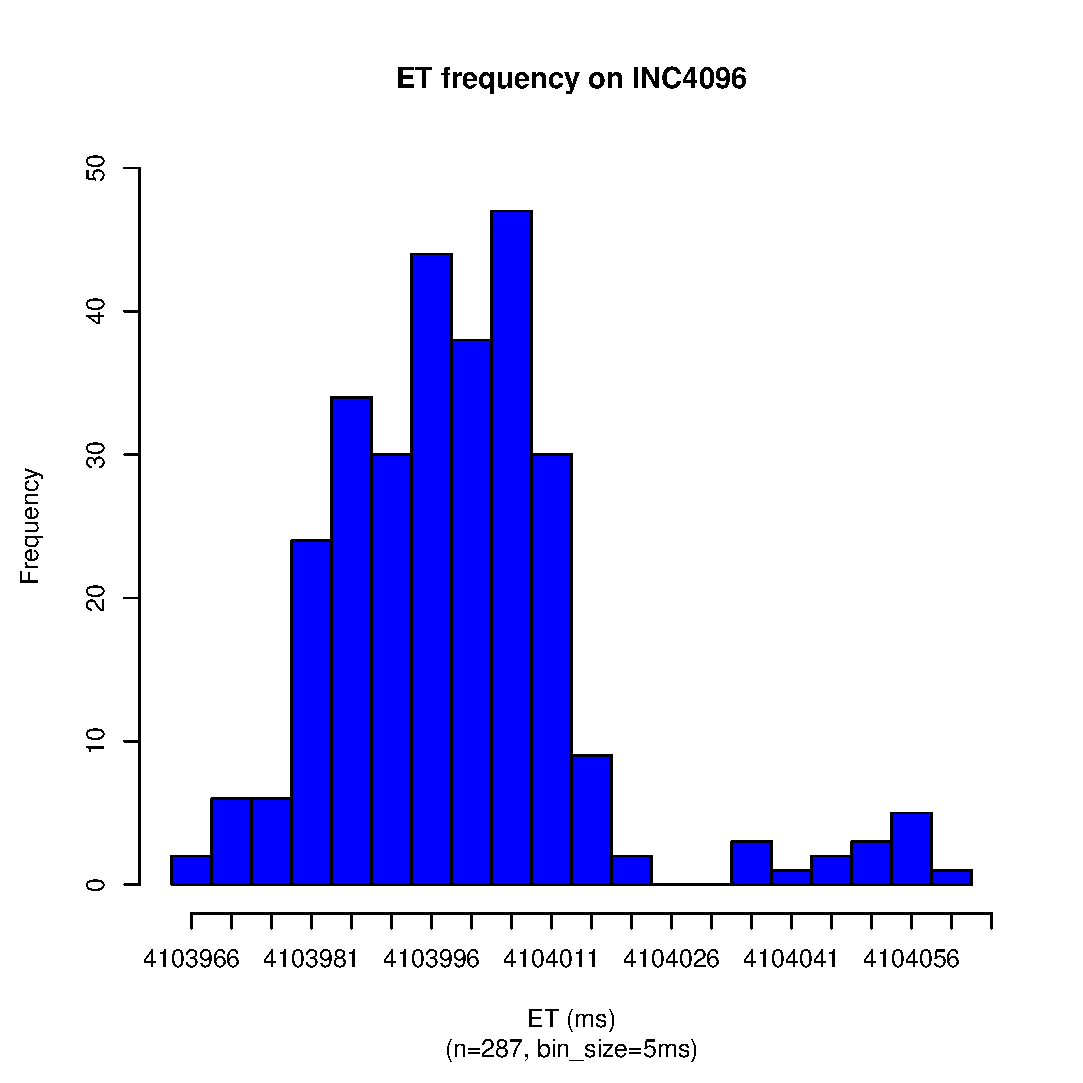
\includegraphics[scale=0.43]{u_s_time/4096_sec_et_hist.eps}
%		\label{fig:inc4096_r3_et_hist_v5}
%	}
%	\caption{ET Histograms of INC2048 ... INC4096~\label{fig:s9_r3_et_hist4}}
%\end{figure}

\vspace\fill
\clearpage

\subsection{PT}

\begin{figure}[hp!]
	\centering
	\subfigure[PT frequency on INC1]{
		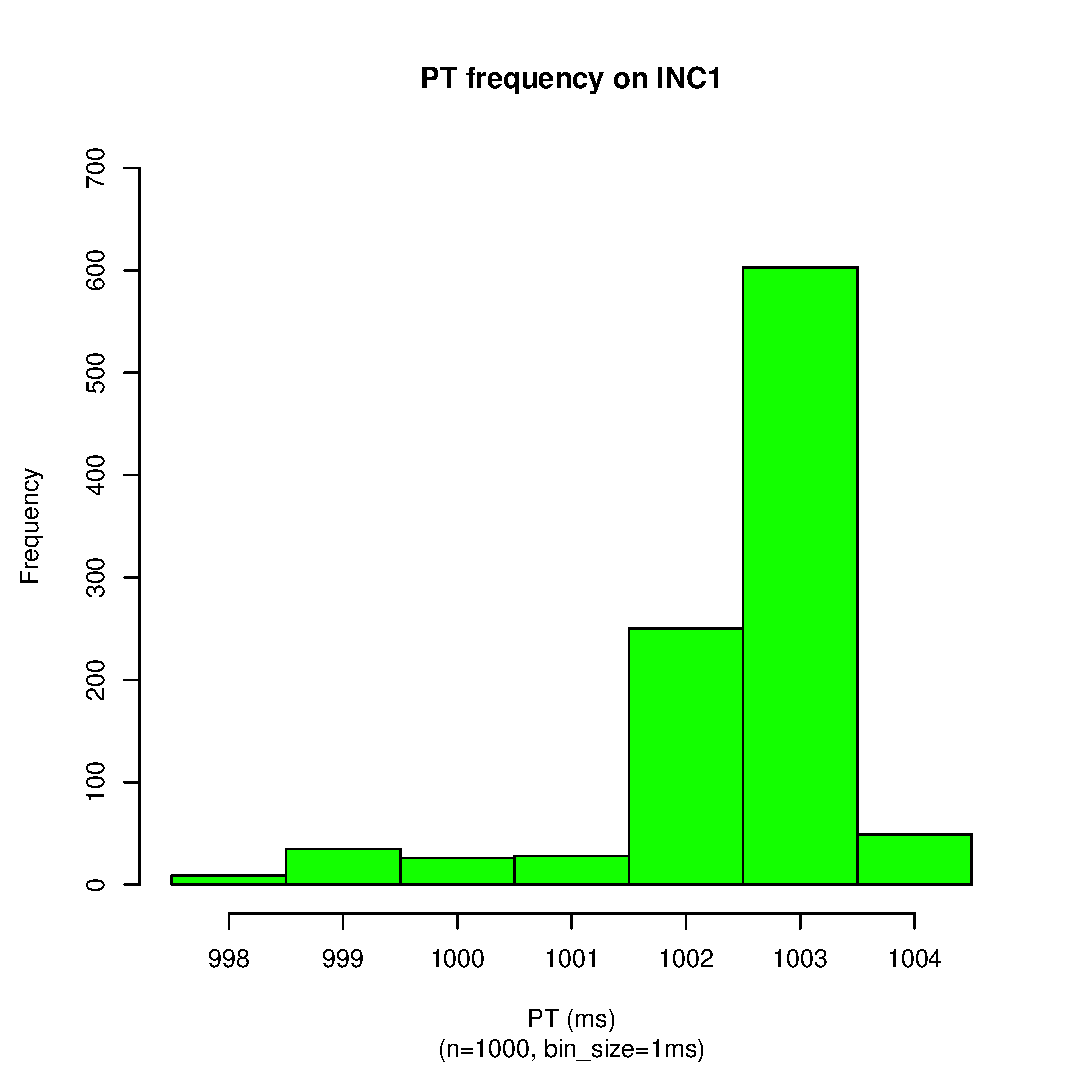
\includegraphics[scale=0.43]{u_s_time/1_sec_pt_hist.eps}
		\label{fig:inc1_r3_hist_v5}
	}
	\subfigure[PT frequency on INC2]{
		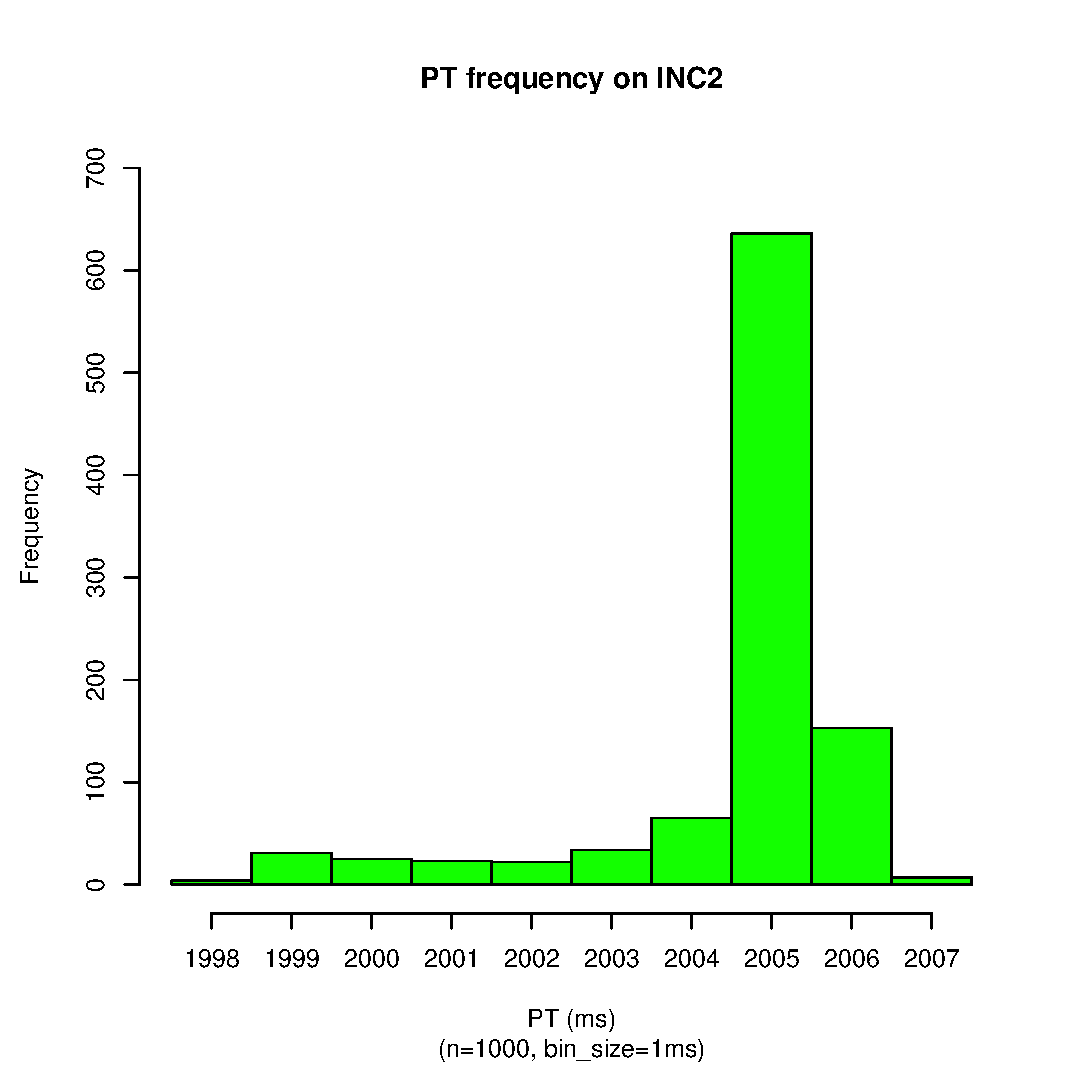
\includegraphics[scale=0.43]{u_s_time/2_sec_pt_hist.eps}
		\label{fig:inc2_r3_hist_v5}
	}
	\subfigure[PT frequency on INC4]{
		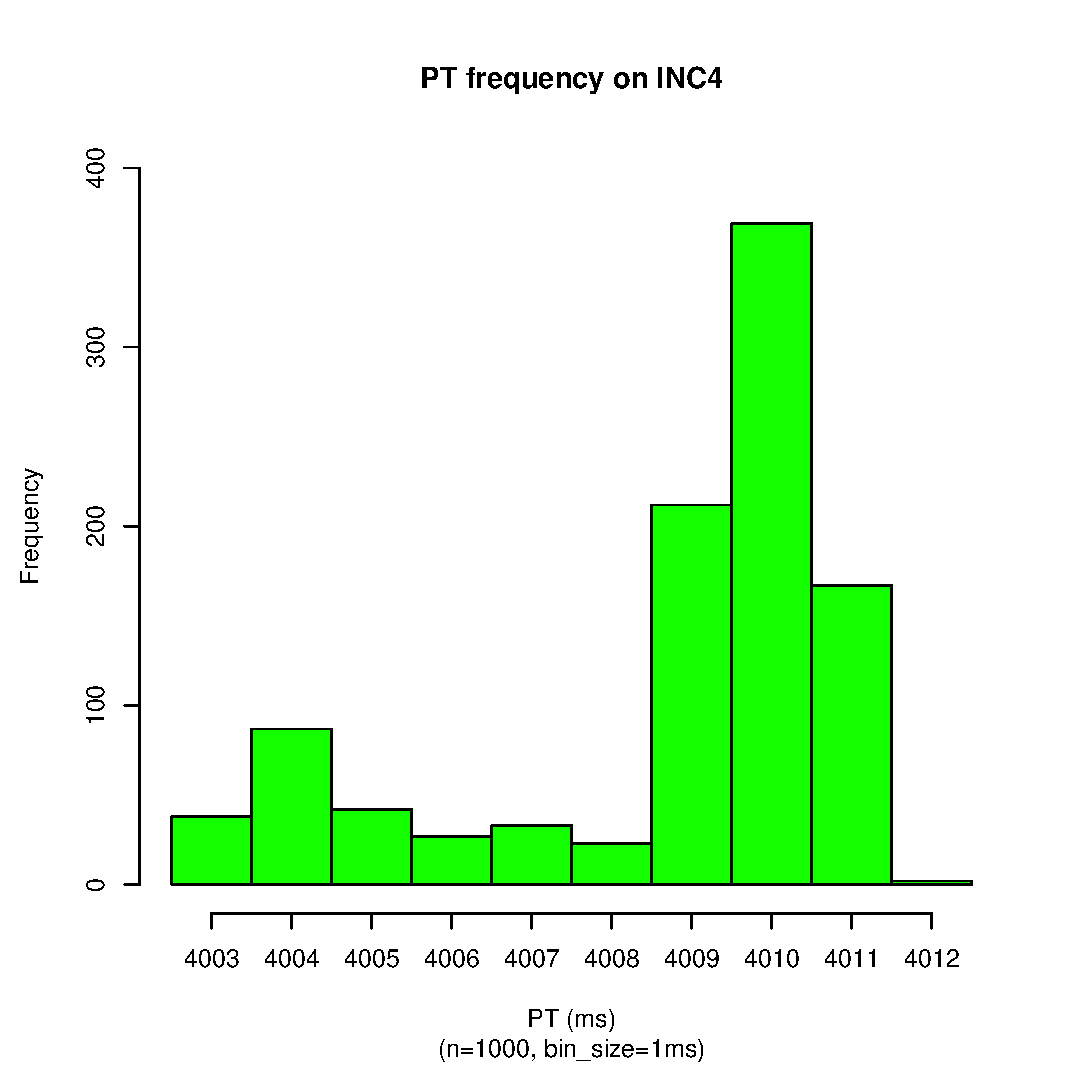
\includegraphics[scale=0.43]{u_s_time/4_sec_pt_hist.eps}
		\label{fig:inc4_r3_hist_v5}
	}
	\subfigure[PT frequency on INC8]{
		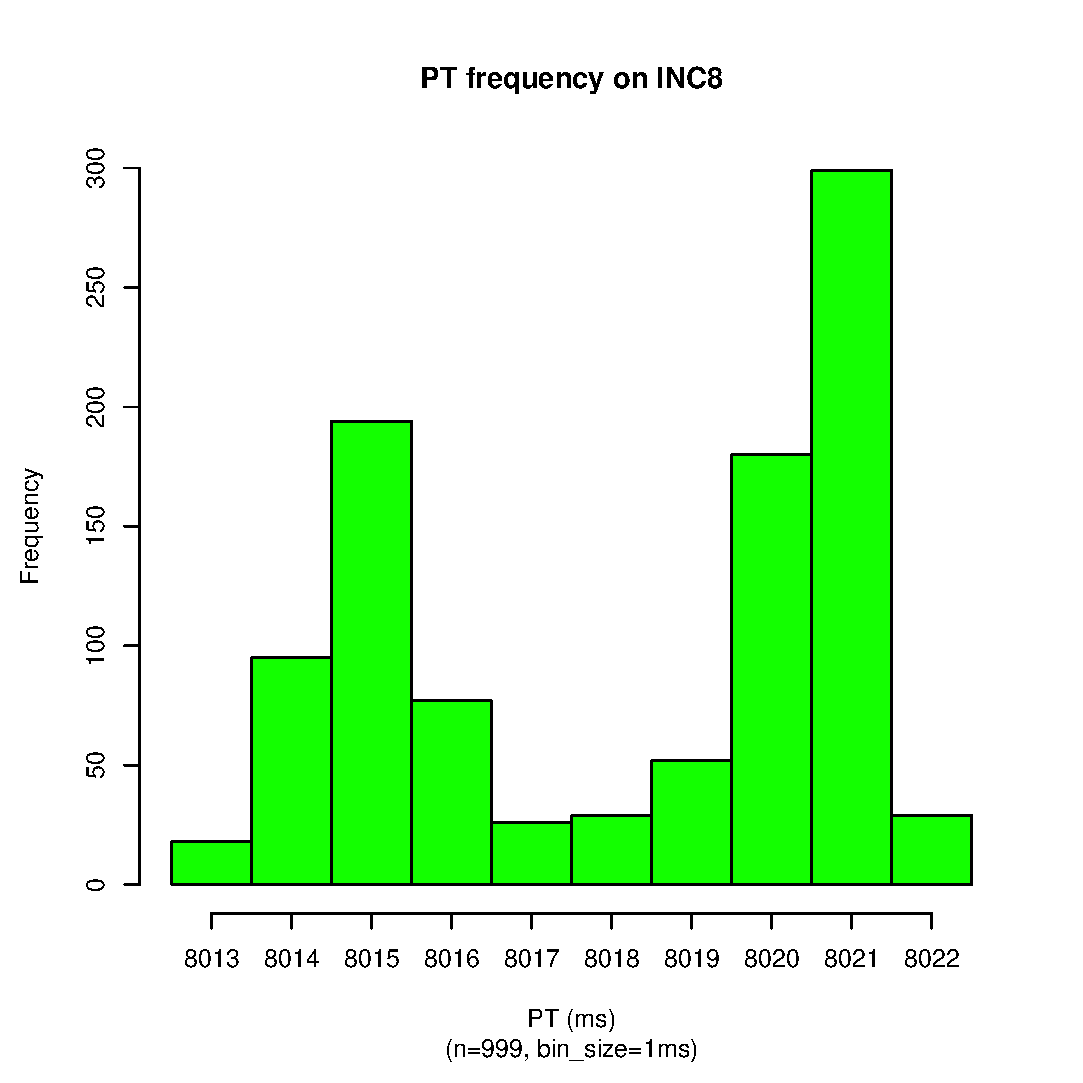
\includegraphics[scale=0.43]{u_s_time/8_sec_pt_hist.eps}
		\label{fig:inc8_r3_hist_v5}
	}
	\caption{PT Histograms of INC1 ... INC8~\label{fig:s9_r3_pt_hist1}}
\end{figure}

\begin{figure}[hp!]
	\centering
	\subfigure[PT frequency on INC16]{
		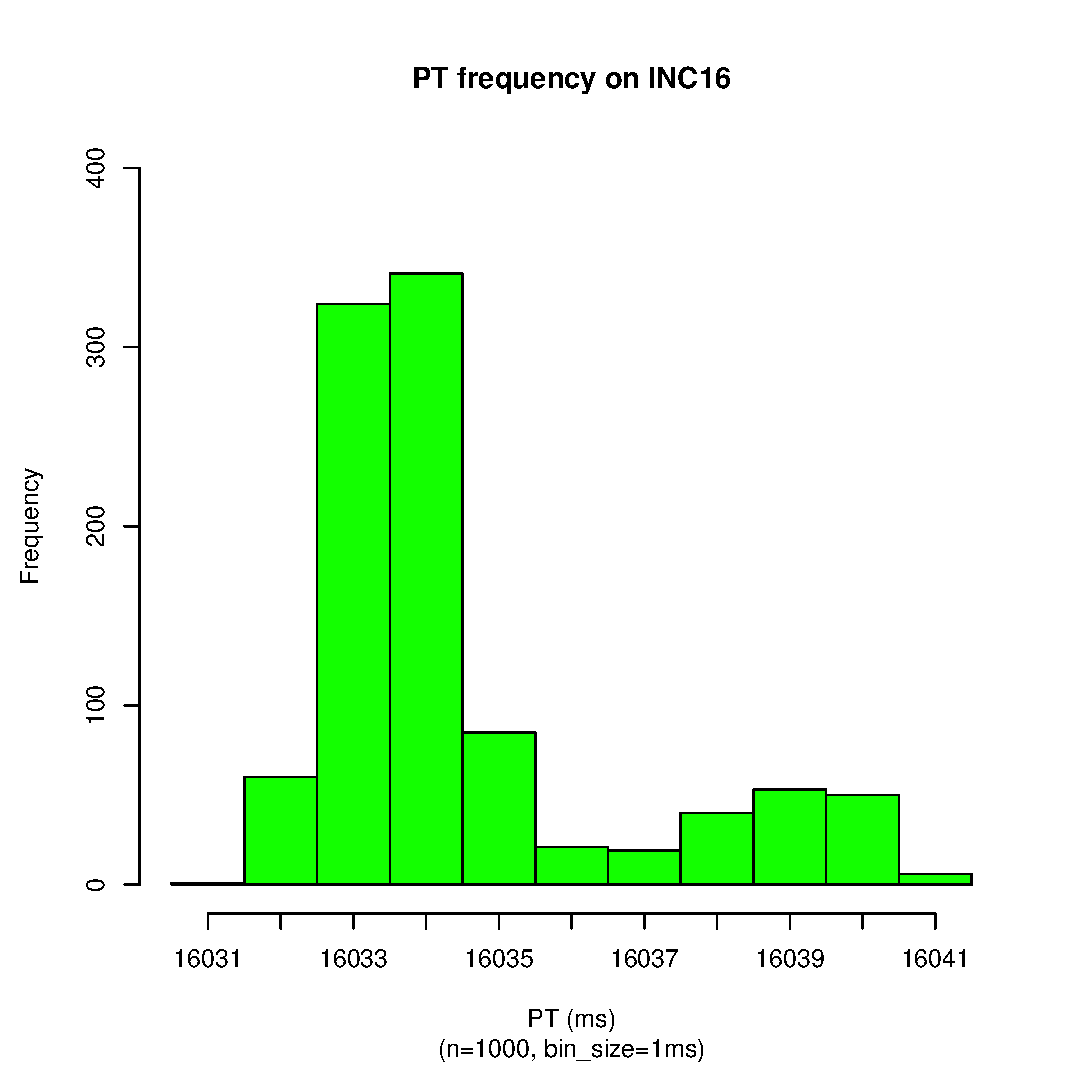
\includegraphics[scale=0.43]{u_s_time/16_sec_pt_hist.eps}
		\label{fig:inc16_r3_hist_v5}
	}
	\subfigure[PT frequency on INC32]{
		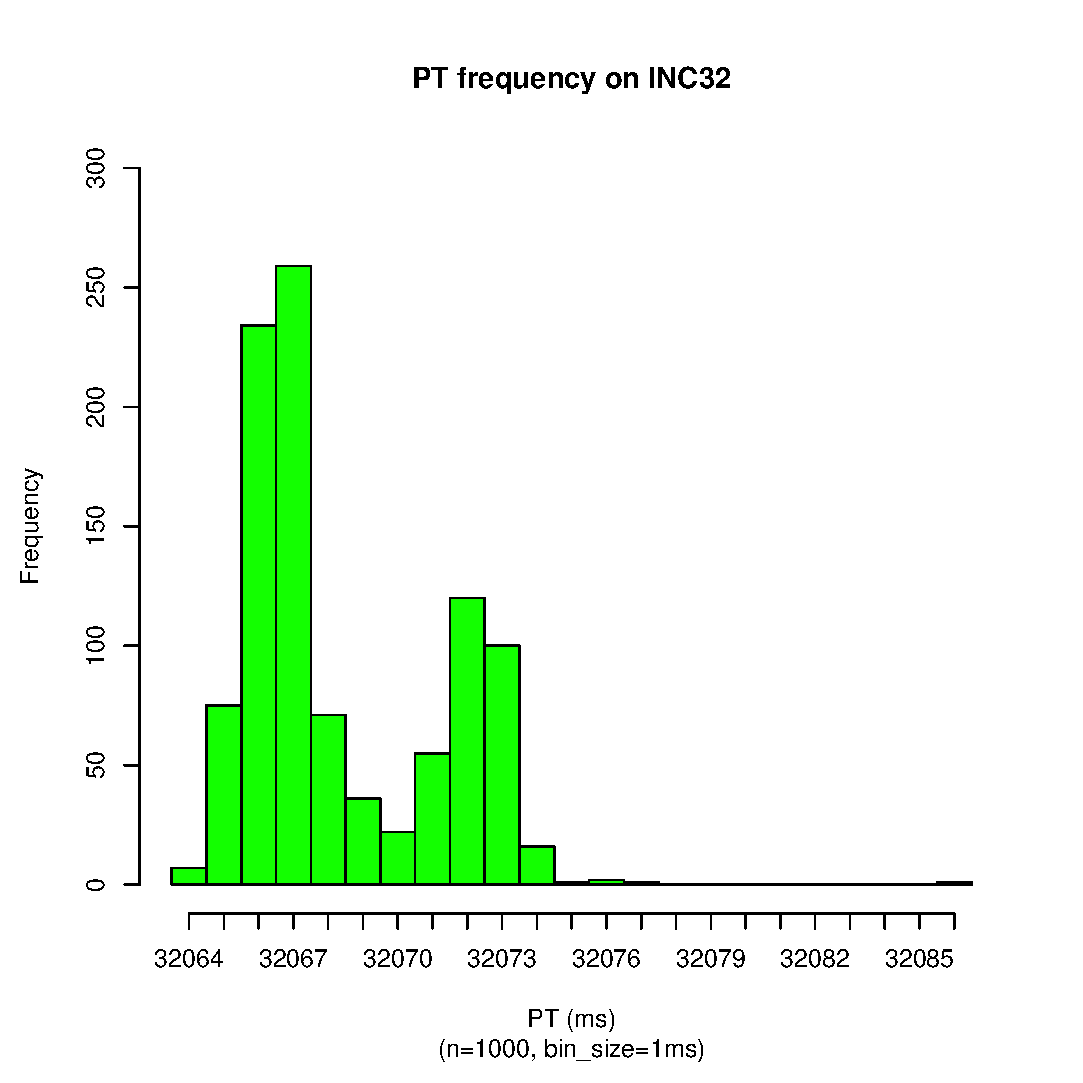
\includegraphics[scale=0.43]{u_s_time/32_sec_pt_hist.eps}
		\label{fig:inc32_r3_hist_v5}
	}
	\subfigure[PT frequency on INC64]{
		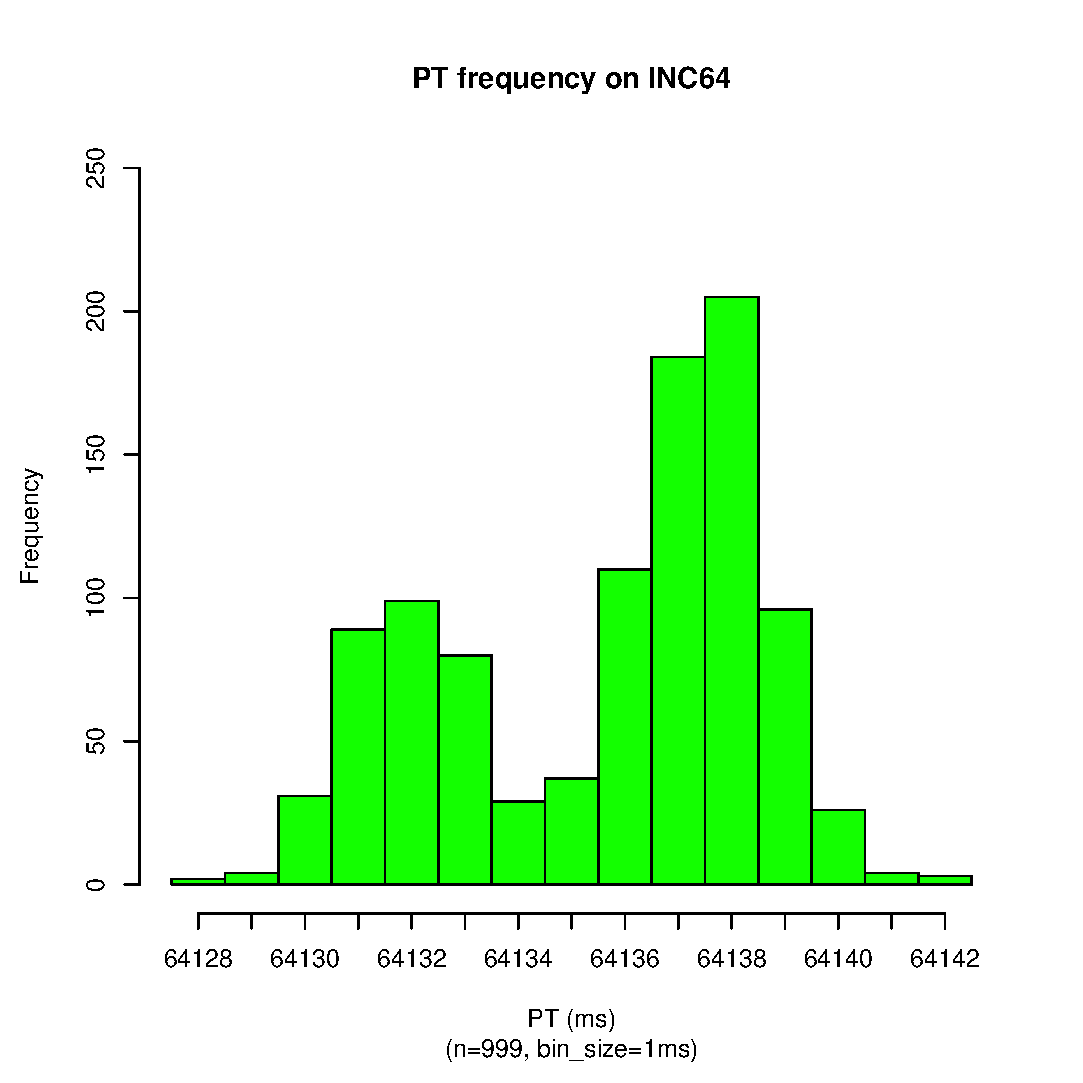
\includegraphics[scale=0.43]{u_s_time/64_sec_pt_hist.eps}
		\label{fig:inc64_r3_hist_v5}
	}
	\caption{PT Histograms of INC16 ... INC64\label{fig:s9_r3_pt_hist2}}
\end{figure}

\begin{figure}[hp!]
	\centering
	\subfigure[PT frequency on INC128]{
		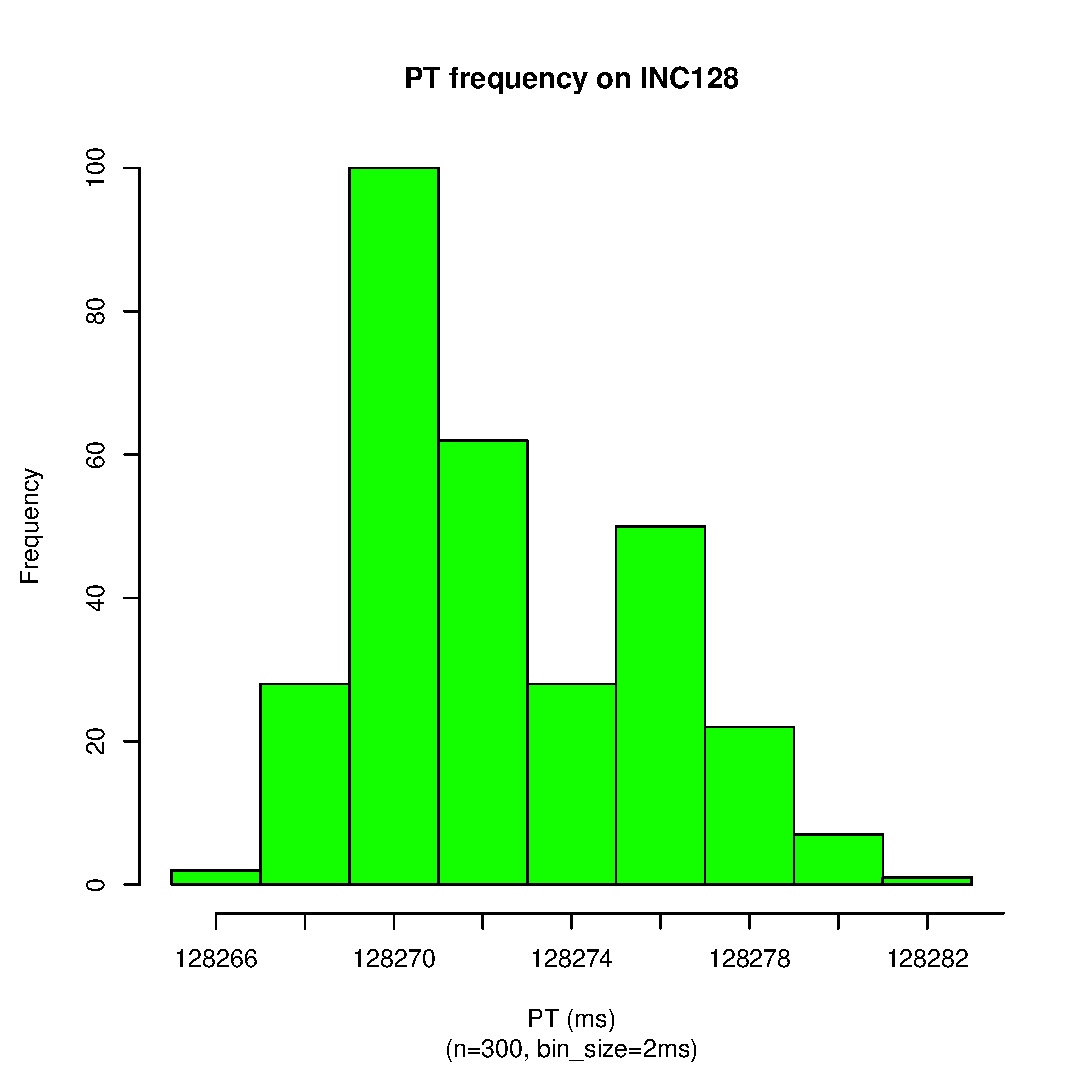
\includegraphics[scale=0.43]{u_s_time/128_sec_pt_hist.eps}
		\label{fig:inc128_r3_hist_v5}
	}
	\subfigure[PT frequency on INC256]{
		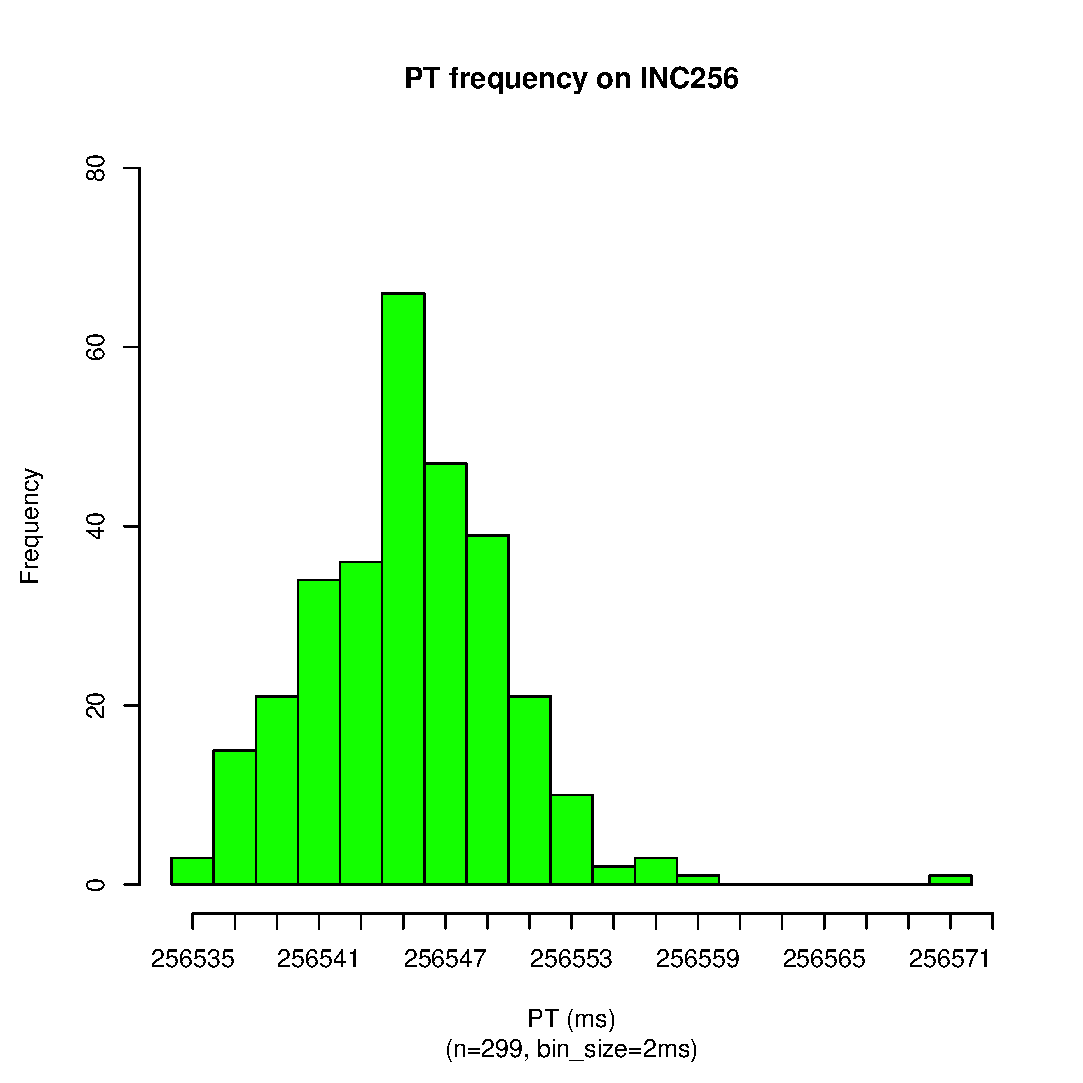
\includegraphics[scale=0.43]{u_s_time/256_sec_pt_hist.eps}
		\label{fig:inc256_r3_hist_v5}
	}
	\subfigure[PT frequency on INC512]{
		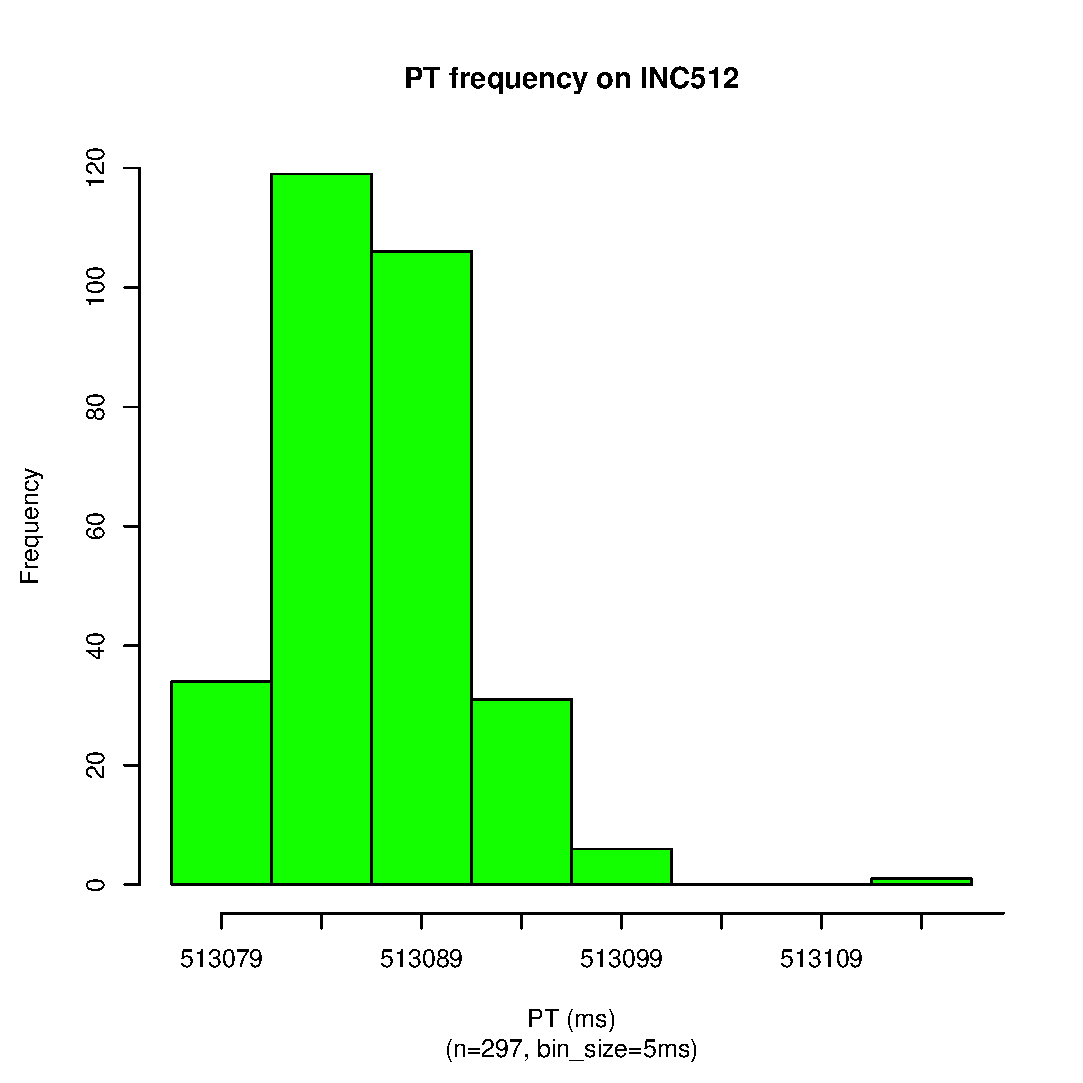
\includegraphics[scale=0.43]{u_s_time/512_sec_pt_hist.eps}
		\label{fig:inc512_r3_hist_v5}
	}
	\subfigure[PT frequency on INC1024]{
		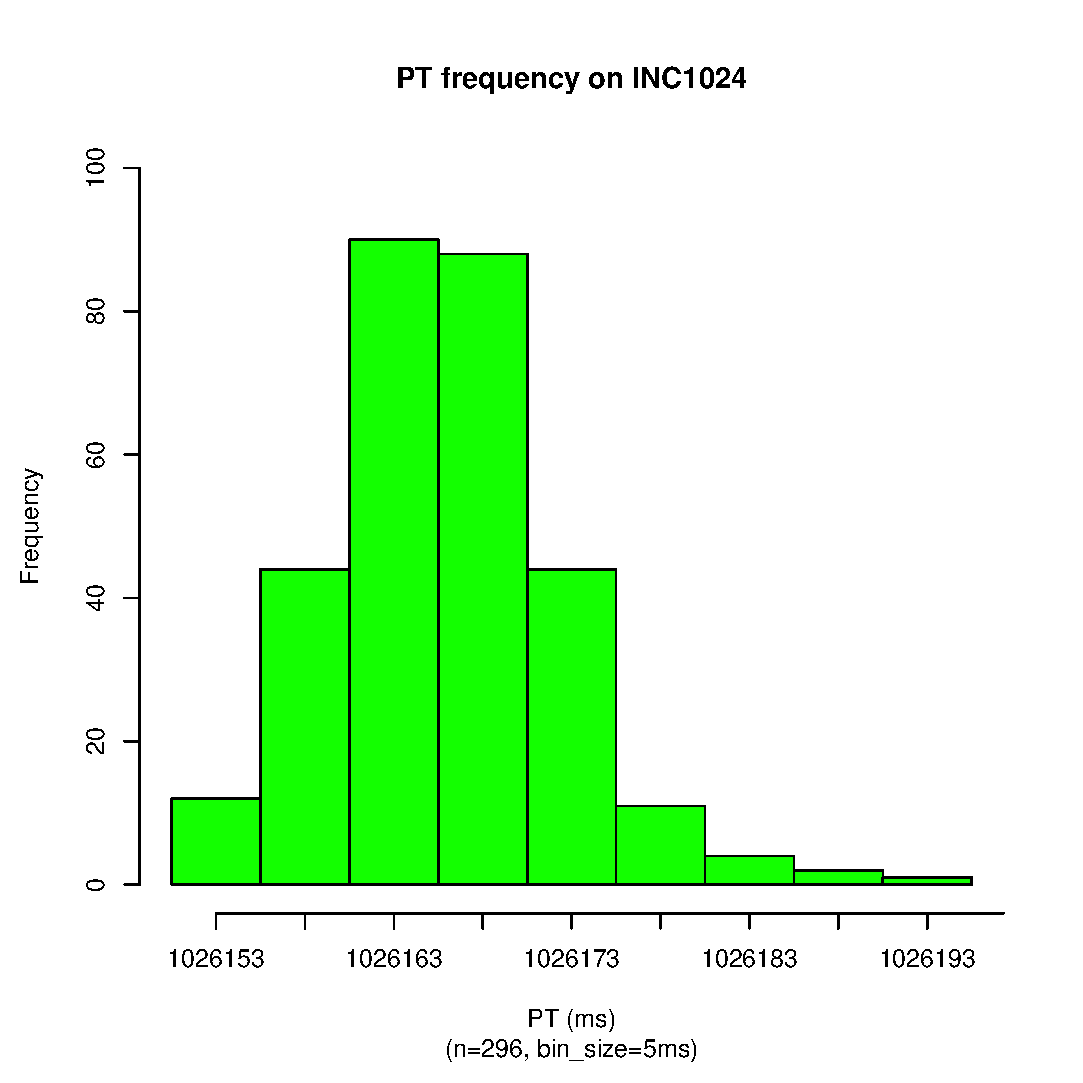
\includegraphics[scale=0.43]{u_s_time/1024_sec_pt_hist.eps}
		\label{fig:inc1024_r3_hist_v5}
	}
	\caption{PT Histograms of INC256 ... INC1024~\label{fig:s9_r3_pt_hist3}}
\end{figure}

%\begin{figure}[t]
%	\centering
%	\subfigure[PT frequency on INC2048]{
%		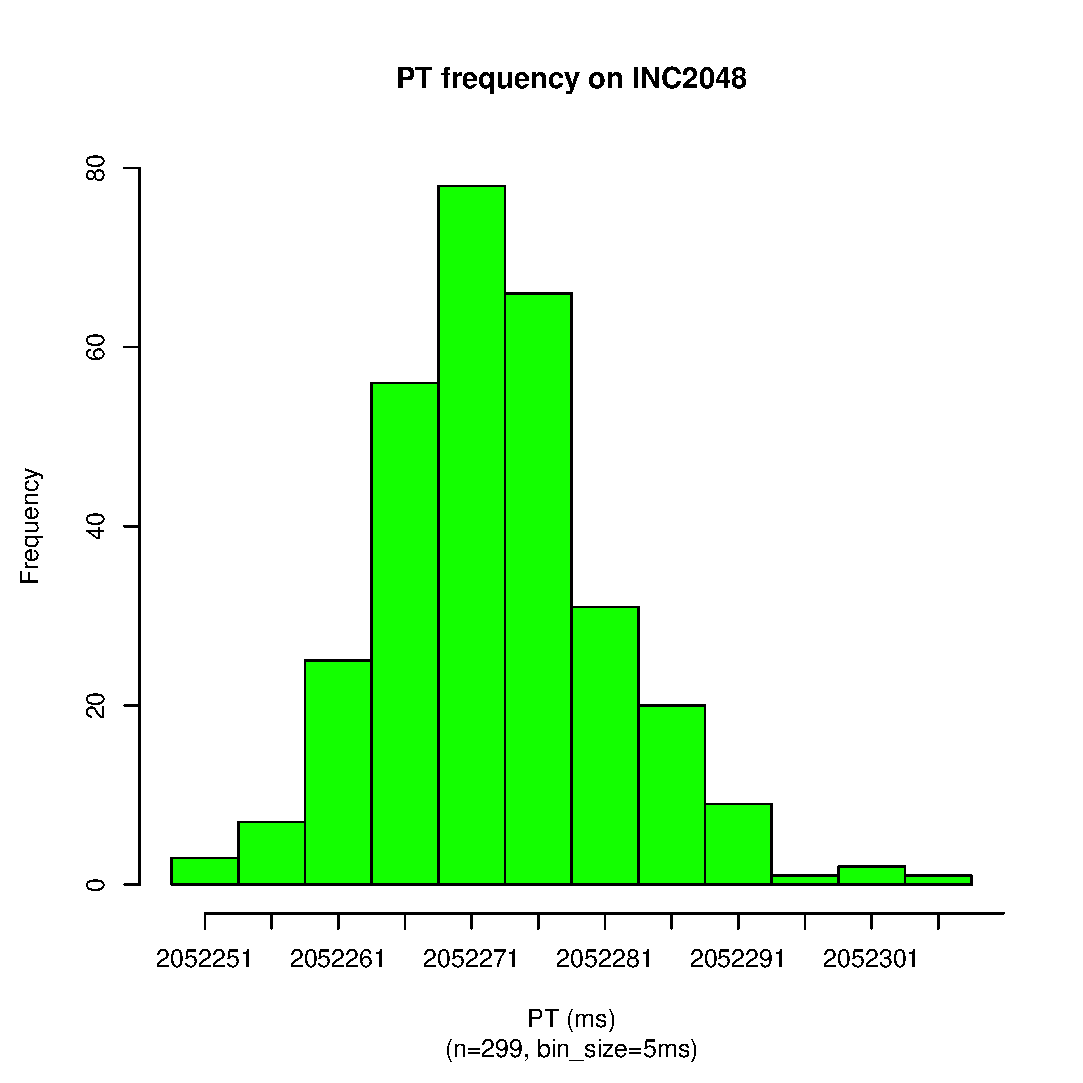
\includegraphics[scale=0.43]{u_s_time/2048_sec_pt_hist.eps}
%		\label{fig:inc2048_r3_hist_v5}
%	}
%	\subfigure[PT frequency on INC4096]{
%		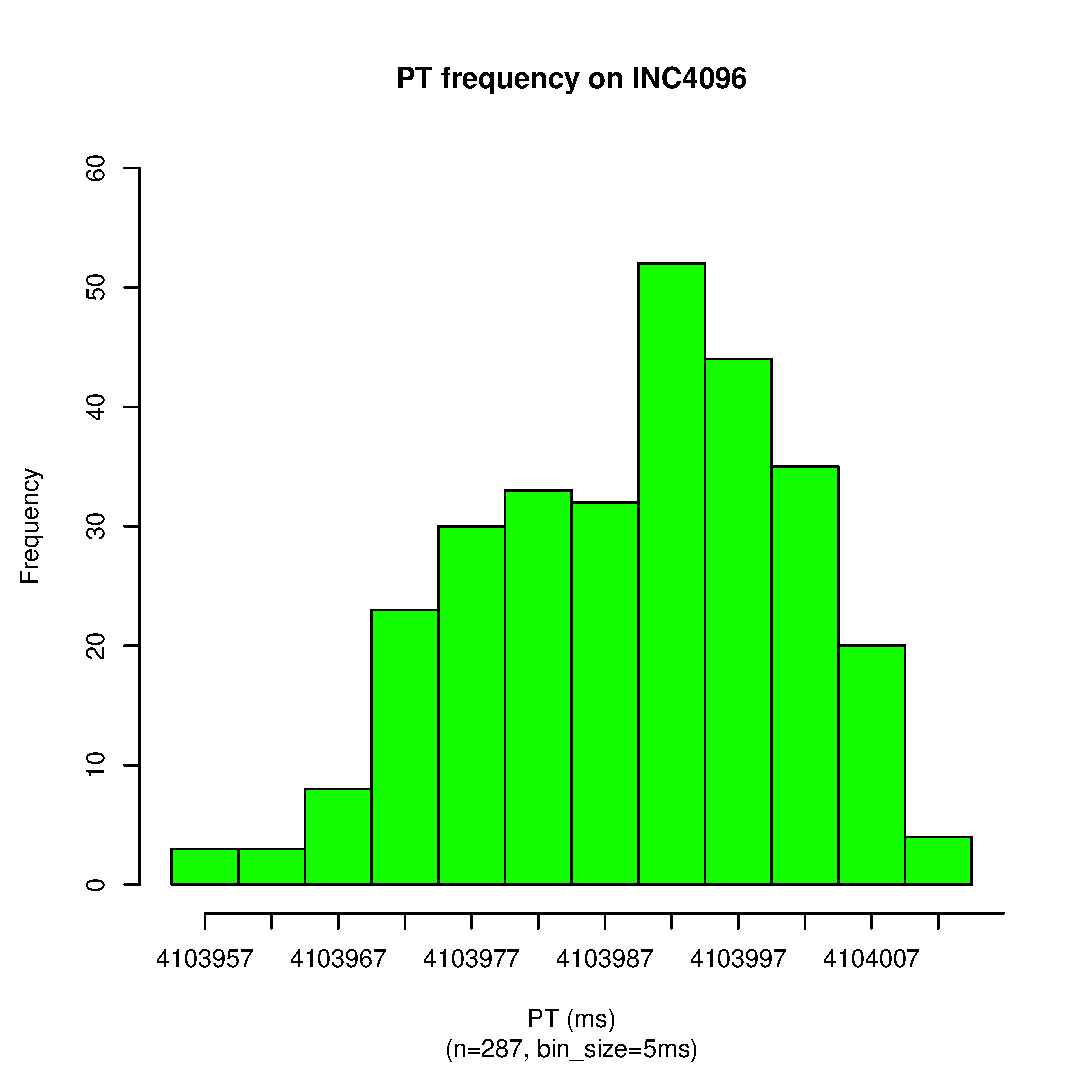
\includegraphics[scale=0.43]{u_s_time/4096_sec_pt_hist.eps}
%		\label{fig:inc4096_r3_hist_v5}
%	}
%%	\subfigure[PT frequency on INC8192]{
%%		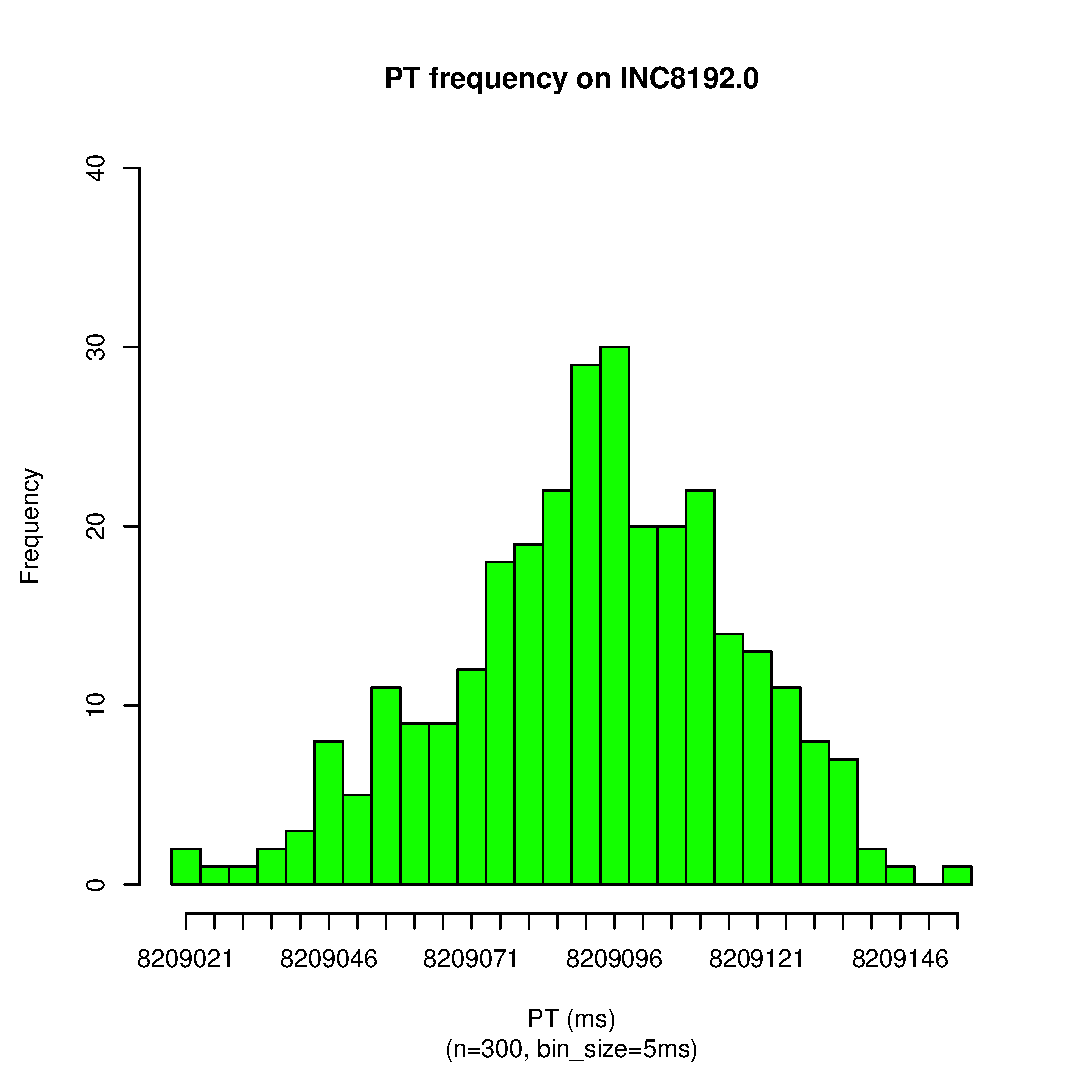
\includegraphics[scale=0.43]{u_s_time/8192_sec_pt_hist.eps}
%%		\label{fig:inc8192_r3_hist_v5}
%%	}
%%	\subfigure[PT frequency on INC16384]{
%%		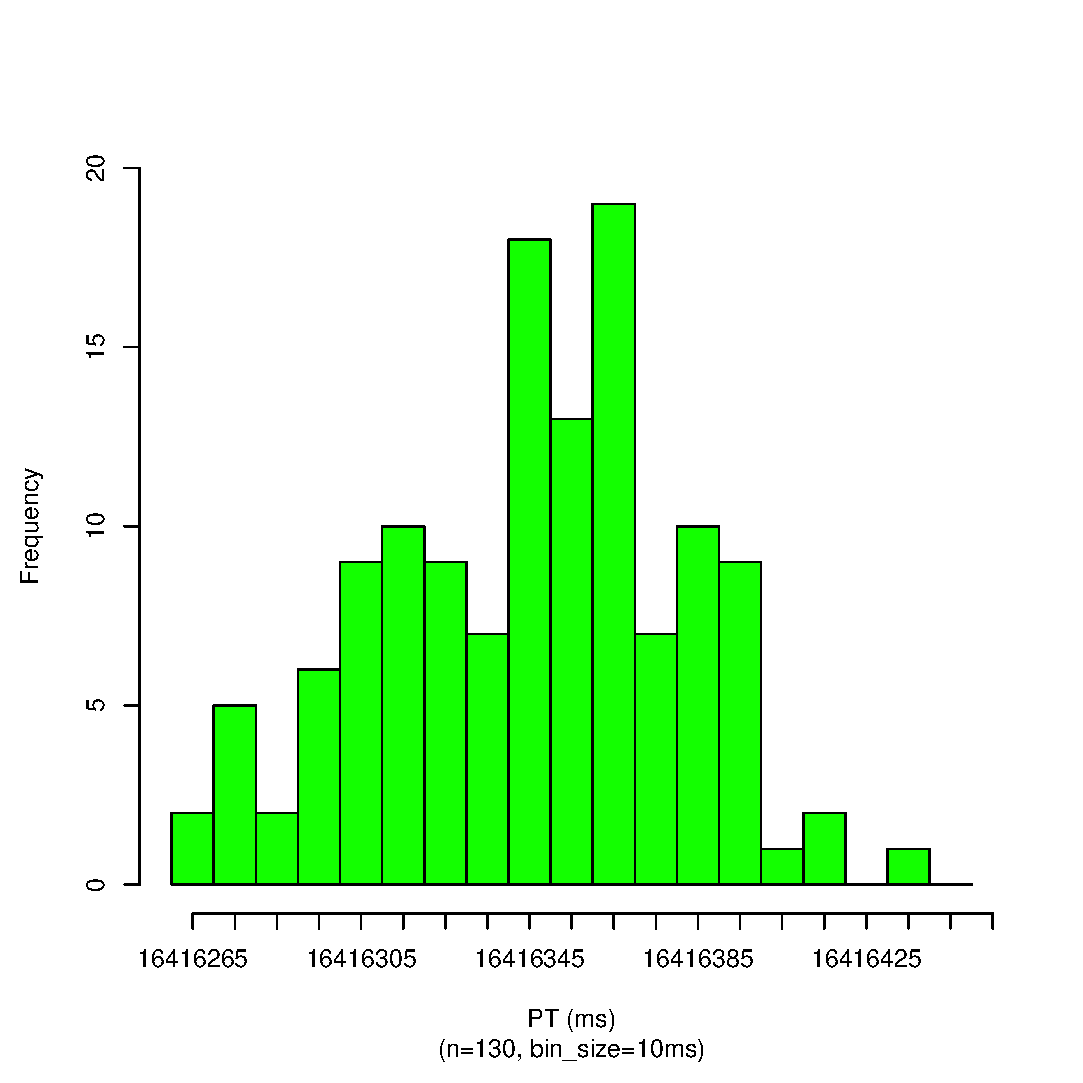
\includegraphics[scale=0.43]{u_s_time/16384_sec_pt_hist.eps}
%%		\label{fig:inc16384_r3_hist_v5}
%%	}
%	\caption{PT Histograms of INC2048 ... INC16384~\label{fig:s9_r3_pt_hist4}}
%\end{figure}

\clearpage
